\documentclass{article}

\usepackage{lipsum}
\usepackage[letterpaper, margin=1.4in]{geometry}
\usepackage{float}
\usepackage{amsmath}
%
\usepackage{tikz}
%
\usetikzlibrary{calc}
%
\usepackage{graphicx}
\usepackage{setspace}
\usepackage{subcaption}
\graphicspath{ {c:/Users/User/Documents/thesis/Thesis/thesisimages/} }


\begin{document}

\begin{titlepage}

\begin{tikzpicture}[overlay,remember picture]
    \draw [line width=1pt,rounded corners=0pt,
        ]
        ($ (current page.north west) + (2cm,-2cm) $)
        rectangle
        ($ (current page.south east) + (-2cm,2cm) $);
\end{tikzpicture}

    \begin{center} 
	\Large
        \vspace*{1cm}
        
        \textbf{ Integrated Deep Learning and Bayesian Classification for Prioritization of Functional Genes in Next-Generation Sequencing Data }
        
        \vspace{0.5cm}
        %subtitle here
        
        \vspace{1.0cm}
        
        \textbf{Chan Khai Ern, Edwin}
        
\vspace{9.0cm}
        \normalsize
       A thesis submitted to the \\
Department of Biochemistry \\
National University of Singapore \\
in partial fulfilment for the \\
Degree of Bachelor of Science with \\Honours
in
Life Sciences\\

        
        \vspace{1.5cm}
        
        
        Life Sciences Honours Cohort \\
        AY2015/2016 S1\\
       
        
    \end{center}
\end{titlepage}


\doublespace
\normalsize
\section{Introduction}
Variant calling is a critical step in the identification of mutations in genomes, and is important in downstream applications such as the annotation of mutant genes and the analysis of physiological consequences. However, current variant callers still tend to have low concordances for variants called (O'Rawe et al., 2013; Cornish and Guda, 2015), primarily due to differences in variant calling algorithms and assumptions. Furthermore, these variant callers do not take into account the importance of each variant in the Human metabolic and biochemical pathways. This is critical for clinicians as a clinician should be able to obtain variants that are of clinical significance, enabling them to embark on the best treatment pathway. In this paper, we describe a tool, INSERTNAMEHERE, to integrate data from multiple variant callers, filter true variants and prioritise their importance. This tool uses deep learning for filtering variants, and bayesian updating to determine variants that are the most important.\\

Variant calling primarily involves the use of various statistical and mathematical methods to discover variants, or mutations, in the genome. Calling variants allows the analysis of deviations and differences between the genome of interest and a standard human genome. However, there are still areas for improvement in current variant calling methods, including dealing with different classes of mutations, as well as reducing the number of false positives (Mohiyuddin, et al., 2015; Gézsi et al., 2015). Both these problems fundamentally result from assumptions and implementations of variant callers - certain algorithms are more sensitive and accurate in calling certain classes of mutations, but suffer from inaccuracies in calling other variant types and edge cases. Probabilistic haplotype generating callers (such as GATK's haplotype caller and FreeBayes) tend to be more accurate for SNPs and indels (McKenna et al. 2010; Garrison \& Marth, 2012). They perform de-novo local assembly, where they rebuild small portions of the genome, and subsequently use bayesian analysis to determine the existence of variants. Specifically, they generate short haplotypes of local regions from sampled sequences, and determine (based on the haplotypes and prior probabilities in the reference genome) whether a variant should be called. However, these methods can only handle limited window sizes, preventing the detection of larger structural variants. For these we have to rely on other tools that examine larger segments of the genome (Ning et al., 2009) or use libraries of known mutation regions, and study these breakpoints to check if any mutations have occurred (Gerstein et al., 2015). Due to the heterogenity in mutations, no single caller works best for all classes of mutations, pointing towards a variant calling framework that aggregates data from multiple callers.\\

Indeed, studies have shown low concordances between variant callers themselves, due to their specific implementations and algorithms (Mohiyuddin, et al., 2015; Gézsi et al., 2015). If we consider that each variant caller samples from the same genome but with a different statistical technique, then we can see each variant caller as a mode of data that provides us with a unique piece of information on the genome. Thus, we can generate more accurate calls by aggregating the multi-modal data from various callers, allowing us to cross validate the variants called using multiple techniques.\\

The simplest approach to aggregate data is concordance - if multiple variant callers are able to call a variant, it is most likely to be accurate. However, the precision of such a tool would be poor due to the differential sensitivity of callers to edge cases. This would defeat the purpose of using multiple callers in the first place, as the strength of a combinatorial approach lies in tapping into the sensitivities of different callers. More sophisticated efforts have since been done to use machine learning methods such as Support Vector Machines as a way to integrate variant calling information (Gézsi et al., 2015), and the authors showed that SVMs presented an improvement over concordance based methods. However, with the advent of deep learning techniques and libraries, which have been shown be able to integrate complex multi-modal information to solve problems (Ng et al., 2015), we hypothesize that deep learning can also be used to integrate the information from variant callers.\\

Deep learning is a method of machine learning that involves deep stacks of artificial neural networks. These neural networks were inspired by the way our synapses work in the brain, and are represented in silico by input/output nodes that fire when a certain threshold is reached. Thus, these neural networks are able to simulate learning - by learning from labelled data correlations between inputs and outputs, these networks are able to predict outputs if given a new input. 

\begin{figure}[h]
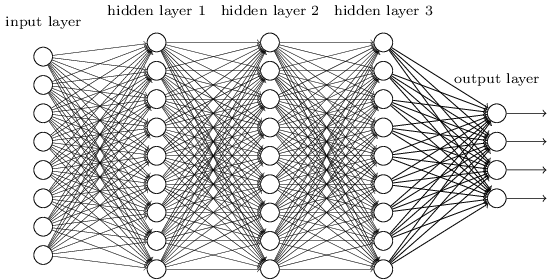
\includegraphics[width=\textwidth]{neuralnet.png}
\centering
\caption{A Neural Network with 1 input layer, 3 hidden layers and 1 output layer. This represents a densely connected neural network, where each node is connected to every node of the preceding and subsequent layers. At each node, linking functions can be had }
\end{figure}

Figure 1 depicts a sample neural network with 5 layers, with 8 data points as input, and 3 data points as output. In such a network, we would train it by providing the input data and output data, and letting the network learn how to integrate the inputs to create a network of activations that can be used to produce the corresponding output. This in part mimics the way we learn - experience teaches us that certain stimuli will result in specific effects (when we see a lightning bolt, we can expect the sound of thunder), and thus when new input comes in (a lightning bolt is seen), we can predict that the output that would arise (thunder is heard). In variant calling, deep learning will allow us to predict based on variant calling patterns and data whether a variant is valid and exists, or is erroneous. This will allow us to draw of the diversity of data with different variant callers, through letting the network learn which patterns will result in a valid call and which patterns are actually false positives. It will also allow us to tap on the differential sensitivity of different callers, as the neural network is able to learn which callers work best for which types of mutations. Thus, such a combinatorial approach will allow us to improve the accuracy and precision of variant calling.\\

\begin{figure}[h]
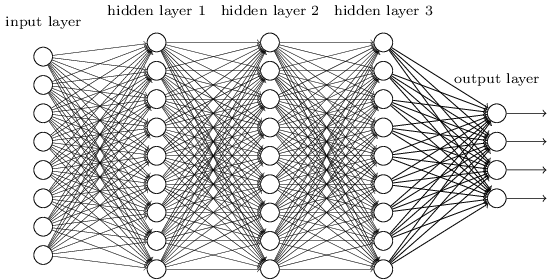
\includegraphics[width=\textwidth]{neuralnet.png}
\centering
\caption{A Neural Network with 1 input layer, 3 hidden layers and 1 output layer. This represents a densely connected neural network, where each node is connected to every node of the preceding and subsequent layers. At each node, linking functions can be had }
\end{figure}


\section{Materials and Methods}

\subsection{Overall Analysis Structure}
Simulate sequence reads with error rates and ground truth variants
Train deep learning neural network using simulated reads to optimize the network
Use optimized network to train on reference genome (NA12878) using high confidence calls as ground truth

Build a Bayesian network based on high confidence calls and functional annotations to rank mutations


\begin{figure}[h]
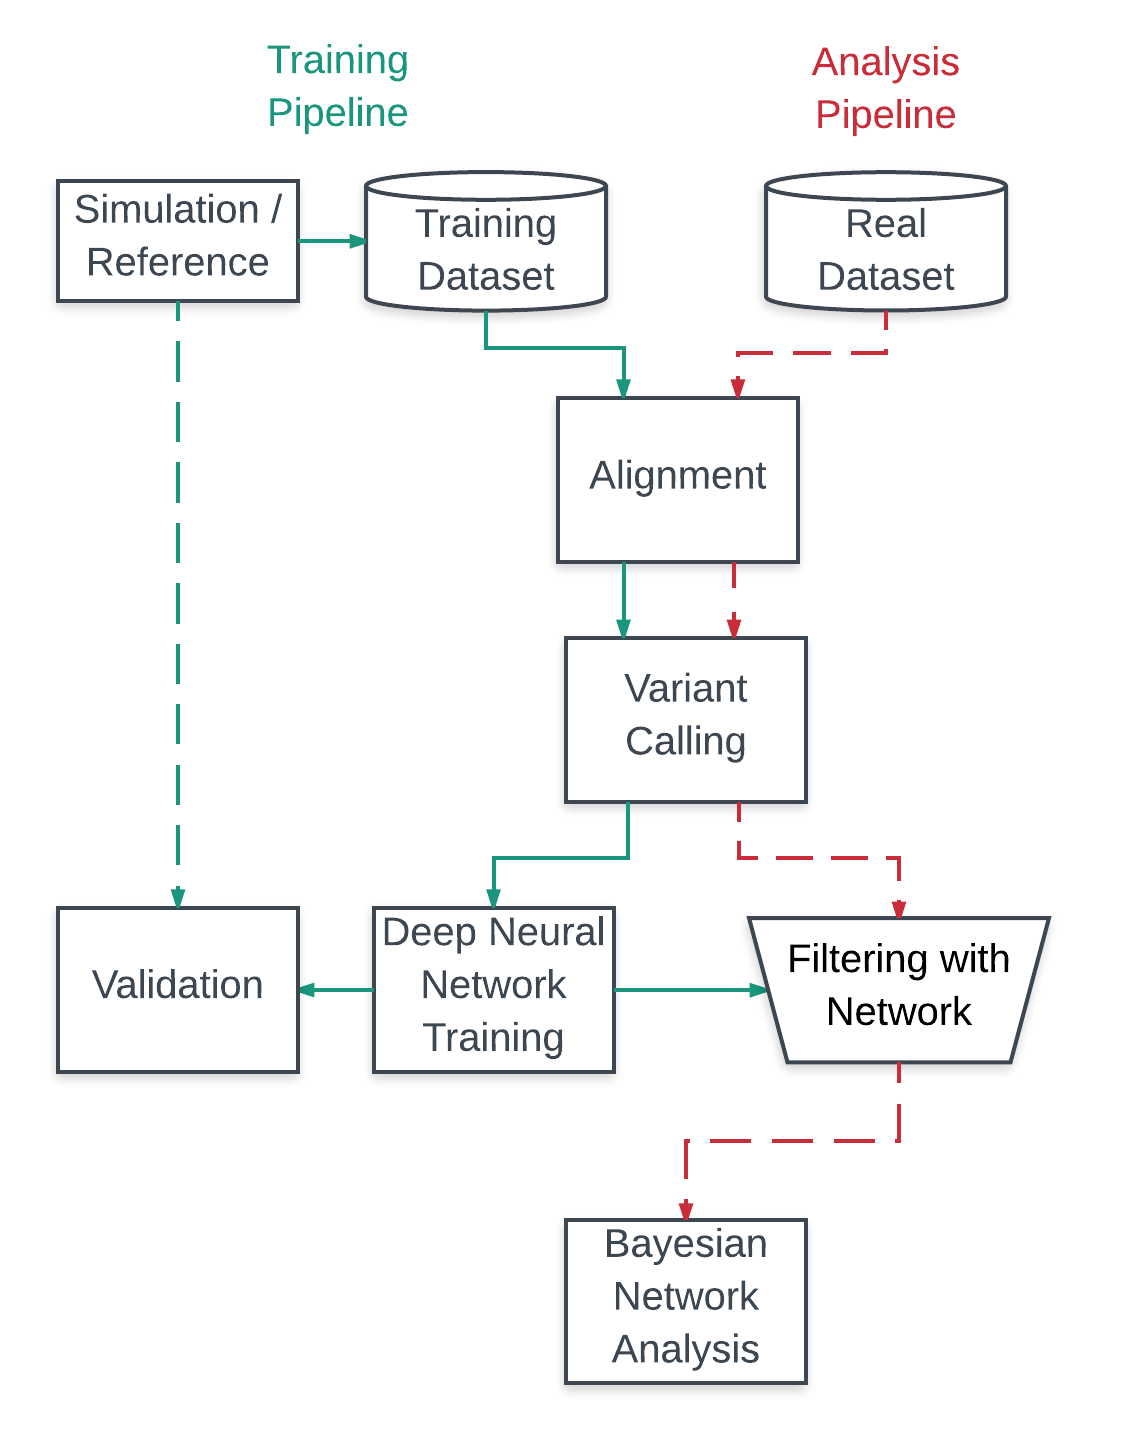
\includegraphics[width=\textwidth]{trainingpathway.png}
\centering
\caption{A Neural Network with 1 input layer, 3 hidden layers and 1 output layer. This represents a densely connected neural network, where each node is connected to every node of the preceding and subsequent layers. At each node, linking functions can be had }
\end{figure}


\subsection{Artificial Datasets}
To generate datasets to train variant calling networks, mason was used in order to generate an artificial genome for analysis. Artificial genomes are the best methods to analyse our neural networks on as the ground truth which are the truth variants inside the genome can be known (CITATION). This allows accurate verification of prediction schemes. It is difficult to obtain complete truth datasets for real genomes as due to the inhibitory cost of checking every variant called. Thus, artificial genomes present a simple way to simulate NGS data with perfectly known ground truth variants to test our validation platform.
To accurately simulate variants, error profiles were obtained from published data (CITATIONS).

\begin{figure}[h]
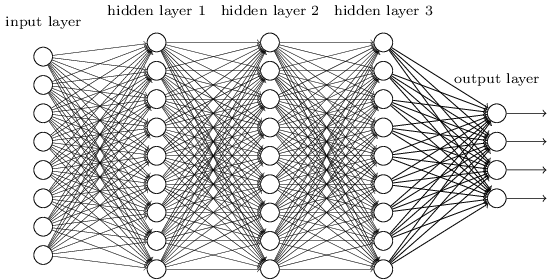
\includegraphics[width=\textwidth]{neuralnet.png}
\centering
\caption{A Neural Network with 1 input layer, 3 hidden layers and 1 output layer. This represents a densely connected neural network, where each node is connected to every node of the preceding and subsequent layers. At each node, linking functions can be had }
\end{figure}


\subsection{Variant Callers}
Variant callers were chosen for our neural network based on their orthogonal calling and reference methodologies - we wanted to maximise the range of variant callers in order to optimise the information that the neural network receives (See Table N). We used two haplotype based callers, FreeBayes (Garrison \& Marth, 2012) and GATK Haplotype Caller (McKenna et al. 2010, DePristo et al. 2011), two position based callers GATK unified Genotyper and Samtools (Li H, et al., 2009) and finally Pindel, a pattern growth based caller (Ye et al., 2009). The features and differences of all 5 callers can be found in Table 1.  All callers have been well studied and are commonly used in variant calling pipelines (Sandmann et al., 2017, Hwang et al., 2015 Xie et al., 2014 and Liu et al., 2013). 

\begin{table}[h]
\caption{Table Comparing Methods and Features of Different variant callers.}
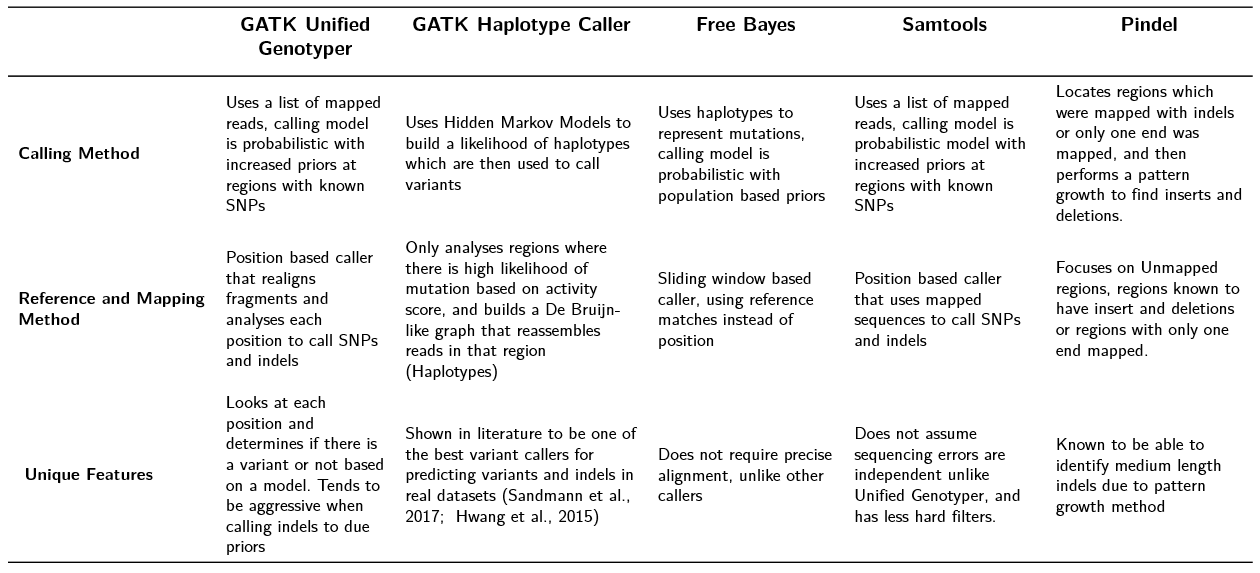
\includegraphics[width=\textwidth]{analysisofvariantcallers.png}
\centering
\end{table}

REFERENCES : \\
Samtools : Li H, et al., 2009\\
GATK UG/HC : McKenna et al. 2010, DePristo et al. 2011\\
FB : Garrison \& Marth, 2012\\
Pindel : Ye et al., 2009\\

\subsection{Feature Selection}

\subsection{Neural Networks}



\subsection{Technologies}
For our deep learning networks, we used the Keras library with a TensorFlow backend. TensorFlow was chosen due to its superior performance on single machines with multiple cores. On our Ubuntu compute cluster, TensorFlow's distributed CPU computation and queue management system enabled better performance in network training compared to other backend machine learning technologies technologies. For more explanation on the algorithms underpinning deep learning, see Appendix (INSERT) for more information 

The general programming platform used was Python. Python was chosen due to its access to various important libraries, including NumPy, SciPy, Pomegrenate and PyVCF. NumPy was used to prepare input vectors for deep learning training, SciPy was used to perform Principal Component Analysis and Synthetic Minority Oversampling Technique Methods (See Appedndix INSERT) for more information. Pomegranate was used to generate and compute the probabilistic model and ranking system for our Bayesian Network (INSERT see MM methods section N for more information). Finally, PyVCF was used to parse the VCF files into python objects for easy manipulation.

\subsection{Feature Engineering}
In order to train the neural network, features were extracted from the variant callers, as well as engineered from the original dataset. All the features used in the training can be found in table N. More information and descriptions of the mathematics behind the engineered features can be found in appendix INSERT.

\begin{table}[]
\caption{Feature Engineering Table}
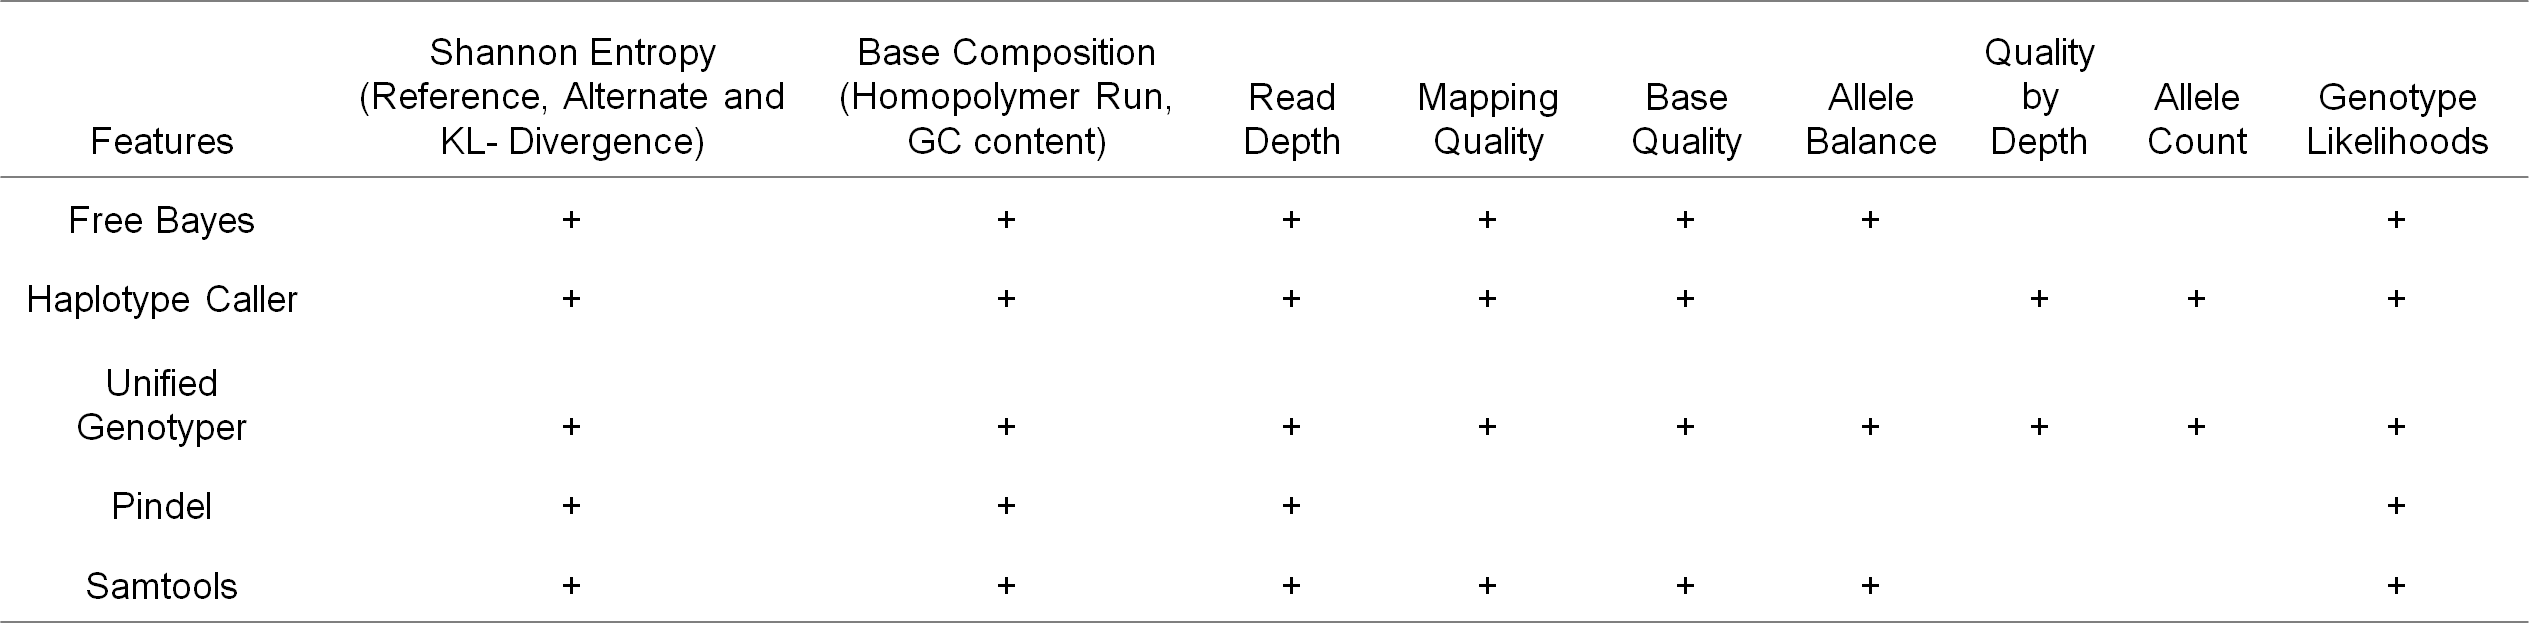
\includegraphics[width=\textwidth]{featureengineering.png}
\centering
\end{table}


\subsection{Artificial Datasets}

\subsection{Processing tools}

\subsection{PDX mouse model development and sequencing}


\section{Results and Discussion}
\subsection{Generation of Artificial Genome}
In order to begin training 

\begin{figure}[H]
\caption{Feature Engineering Table}
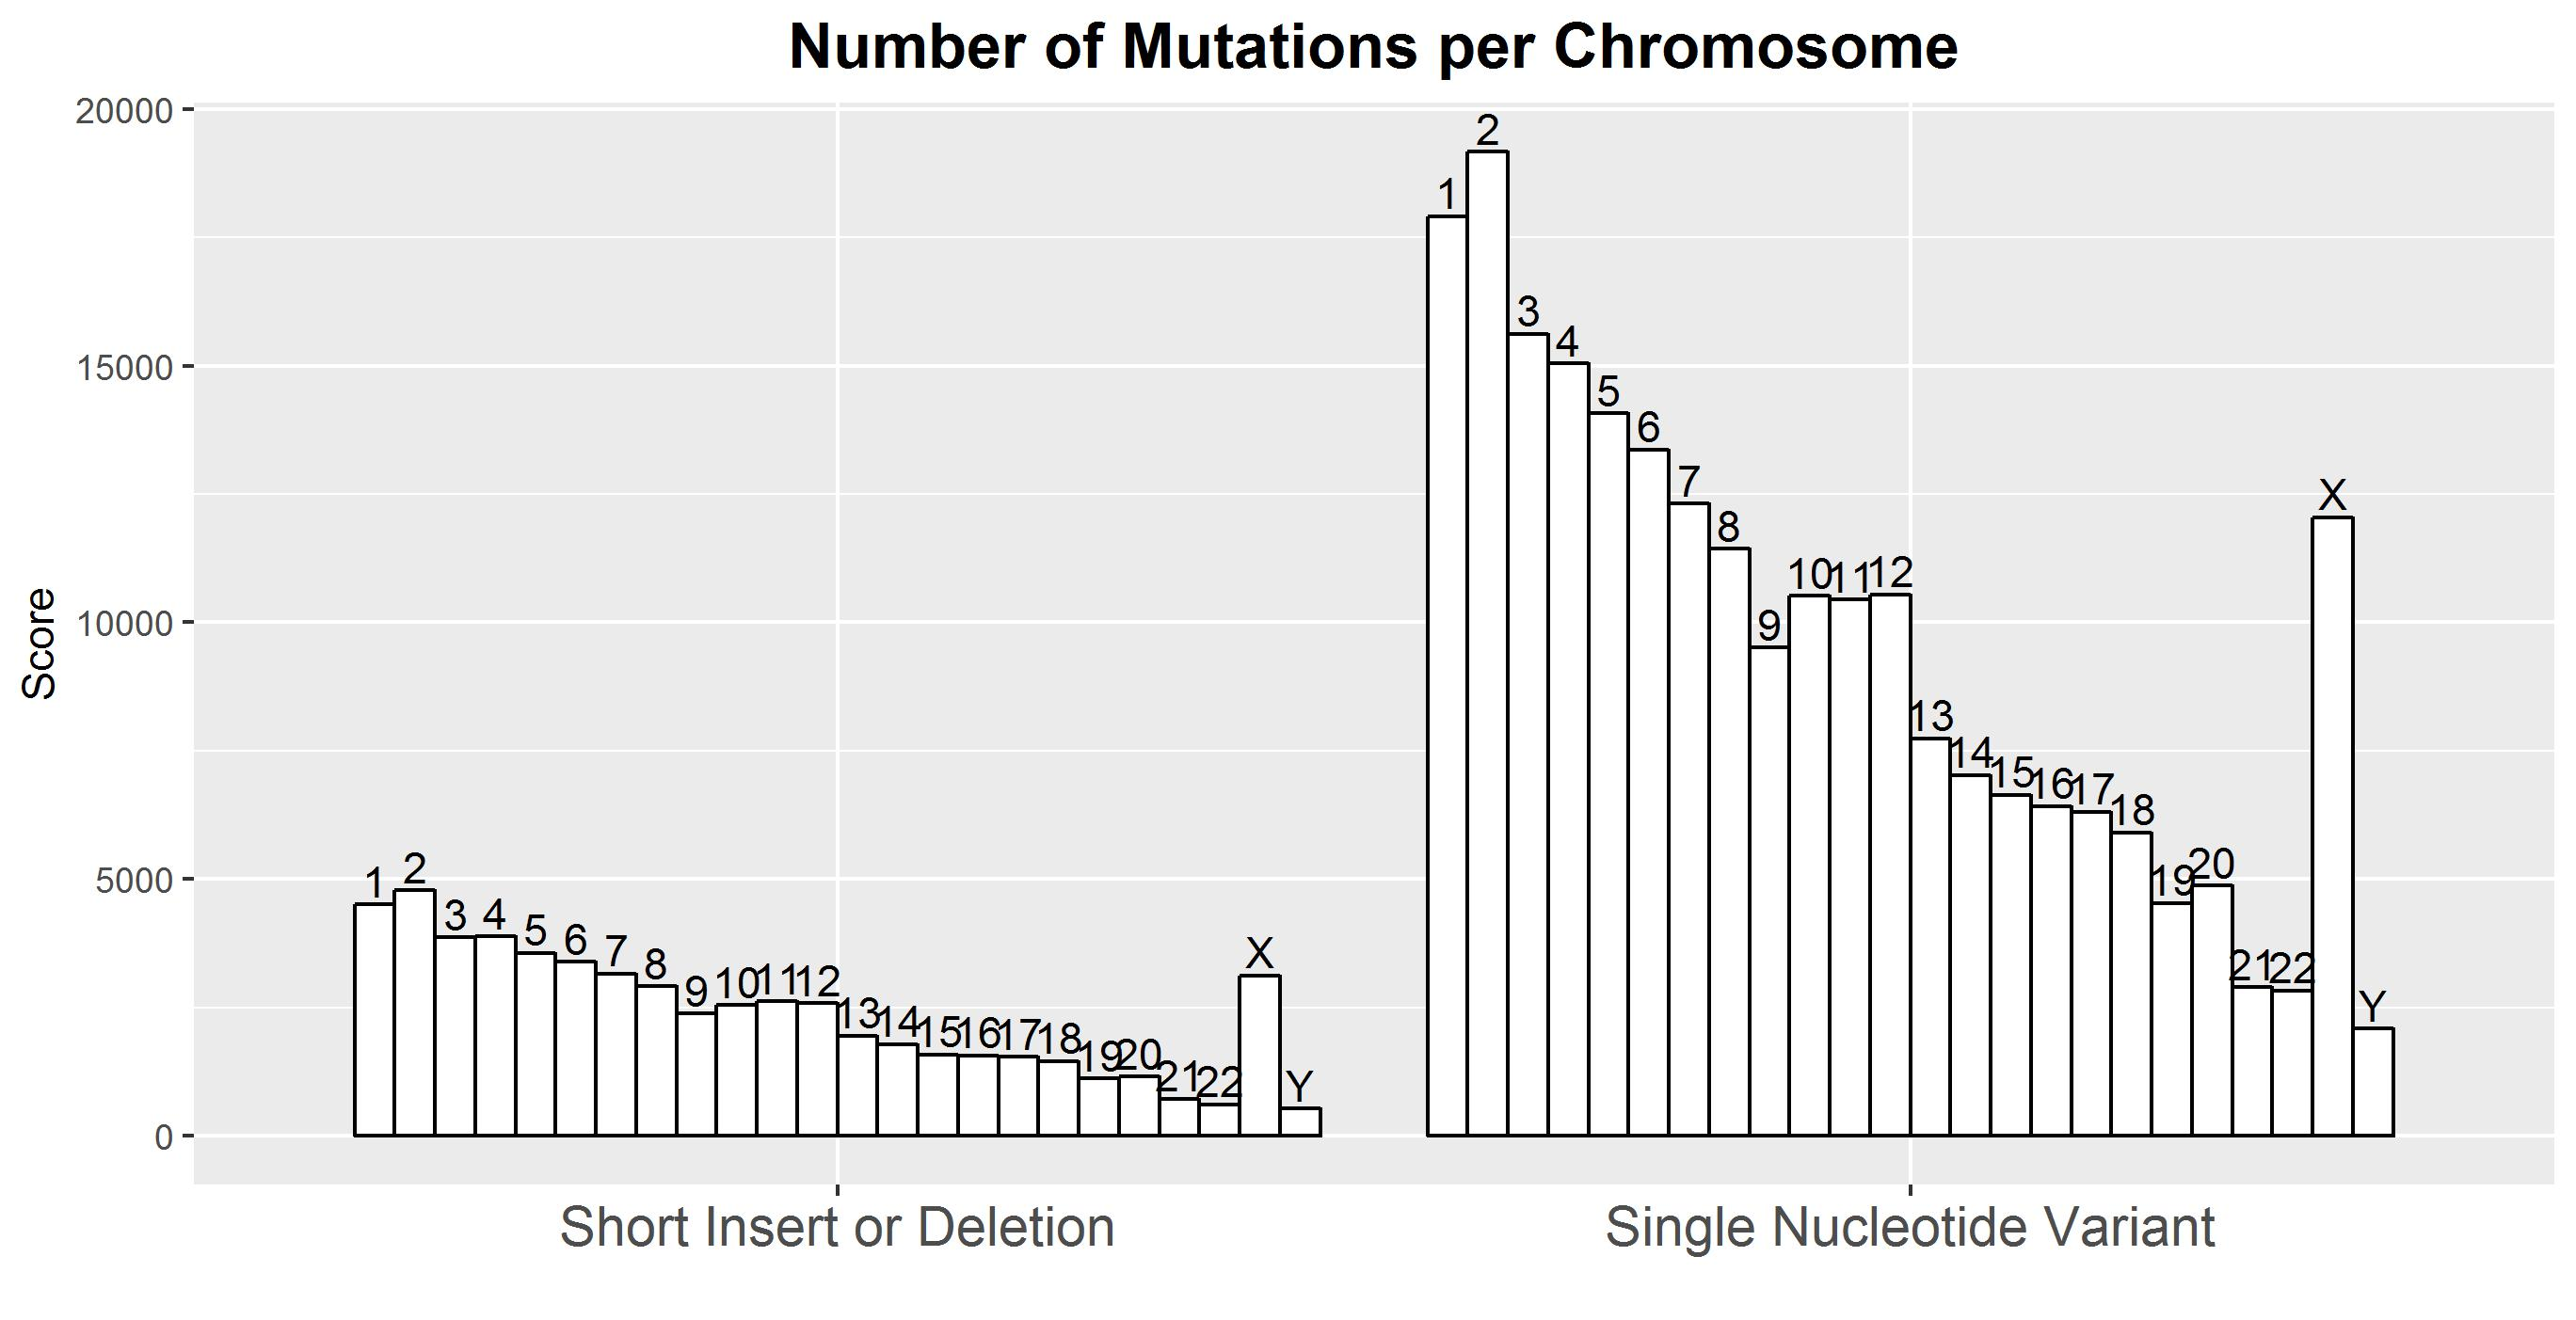
\includegraphics[width=\textwidth]{MutationInSimulatedGenome.jpg}
\centering
\end{figure}

\begin{figure}[H]
\caption{Feature Engineering Table}
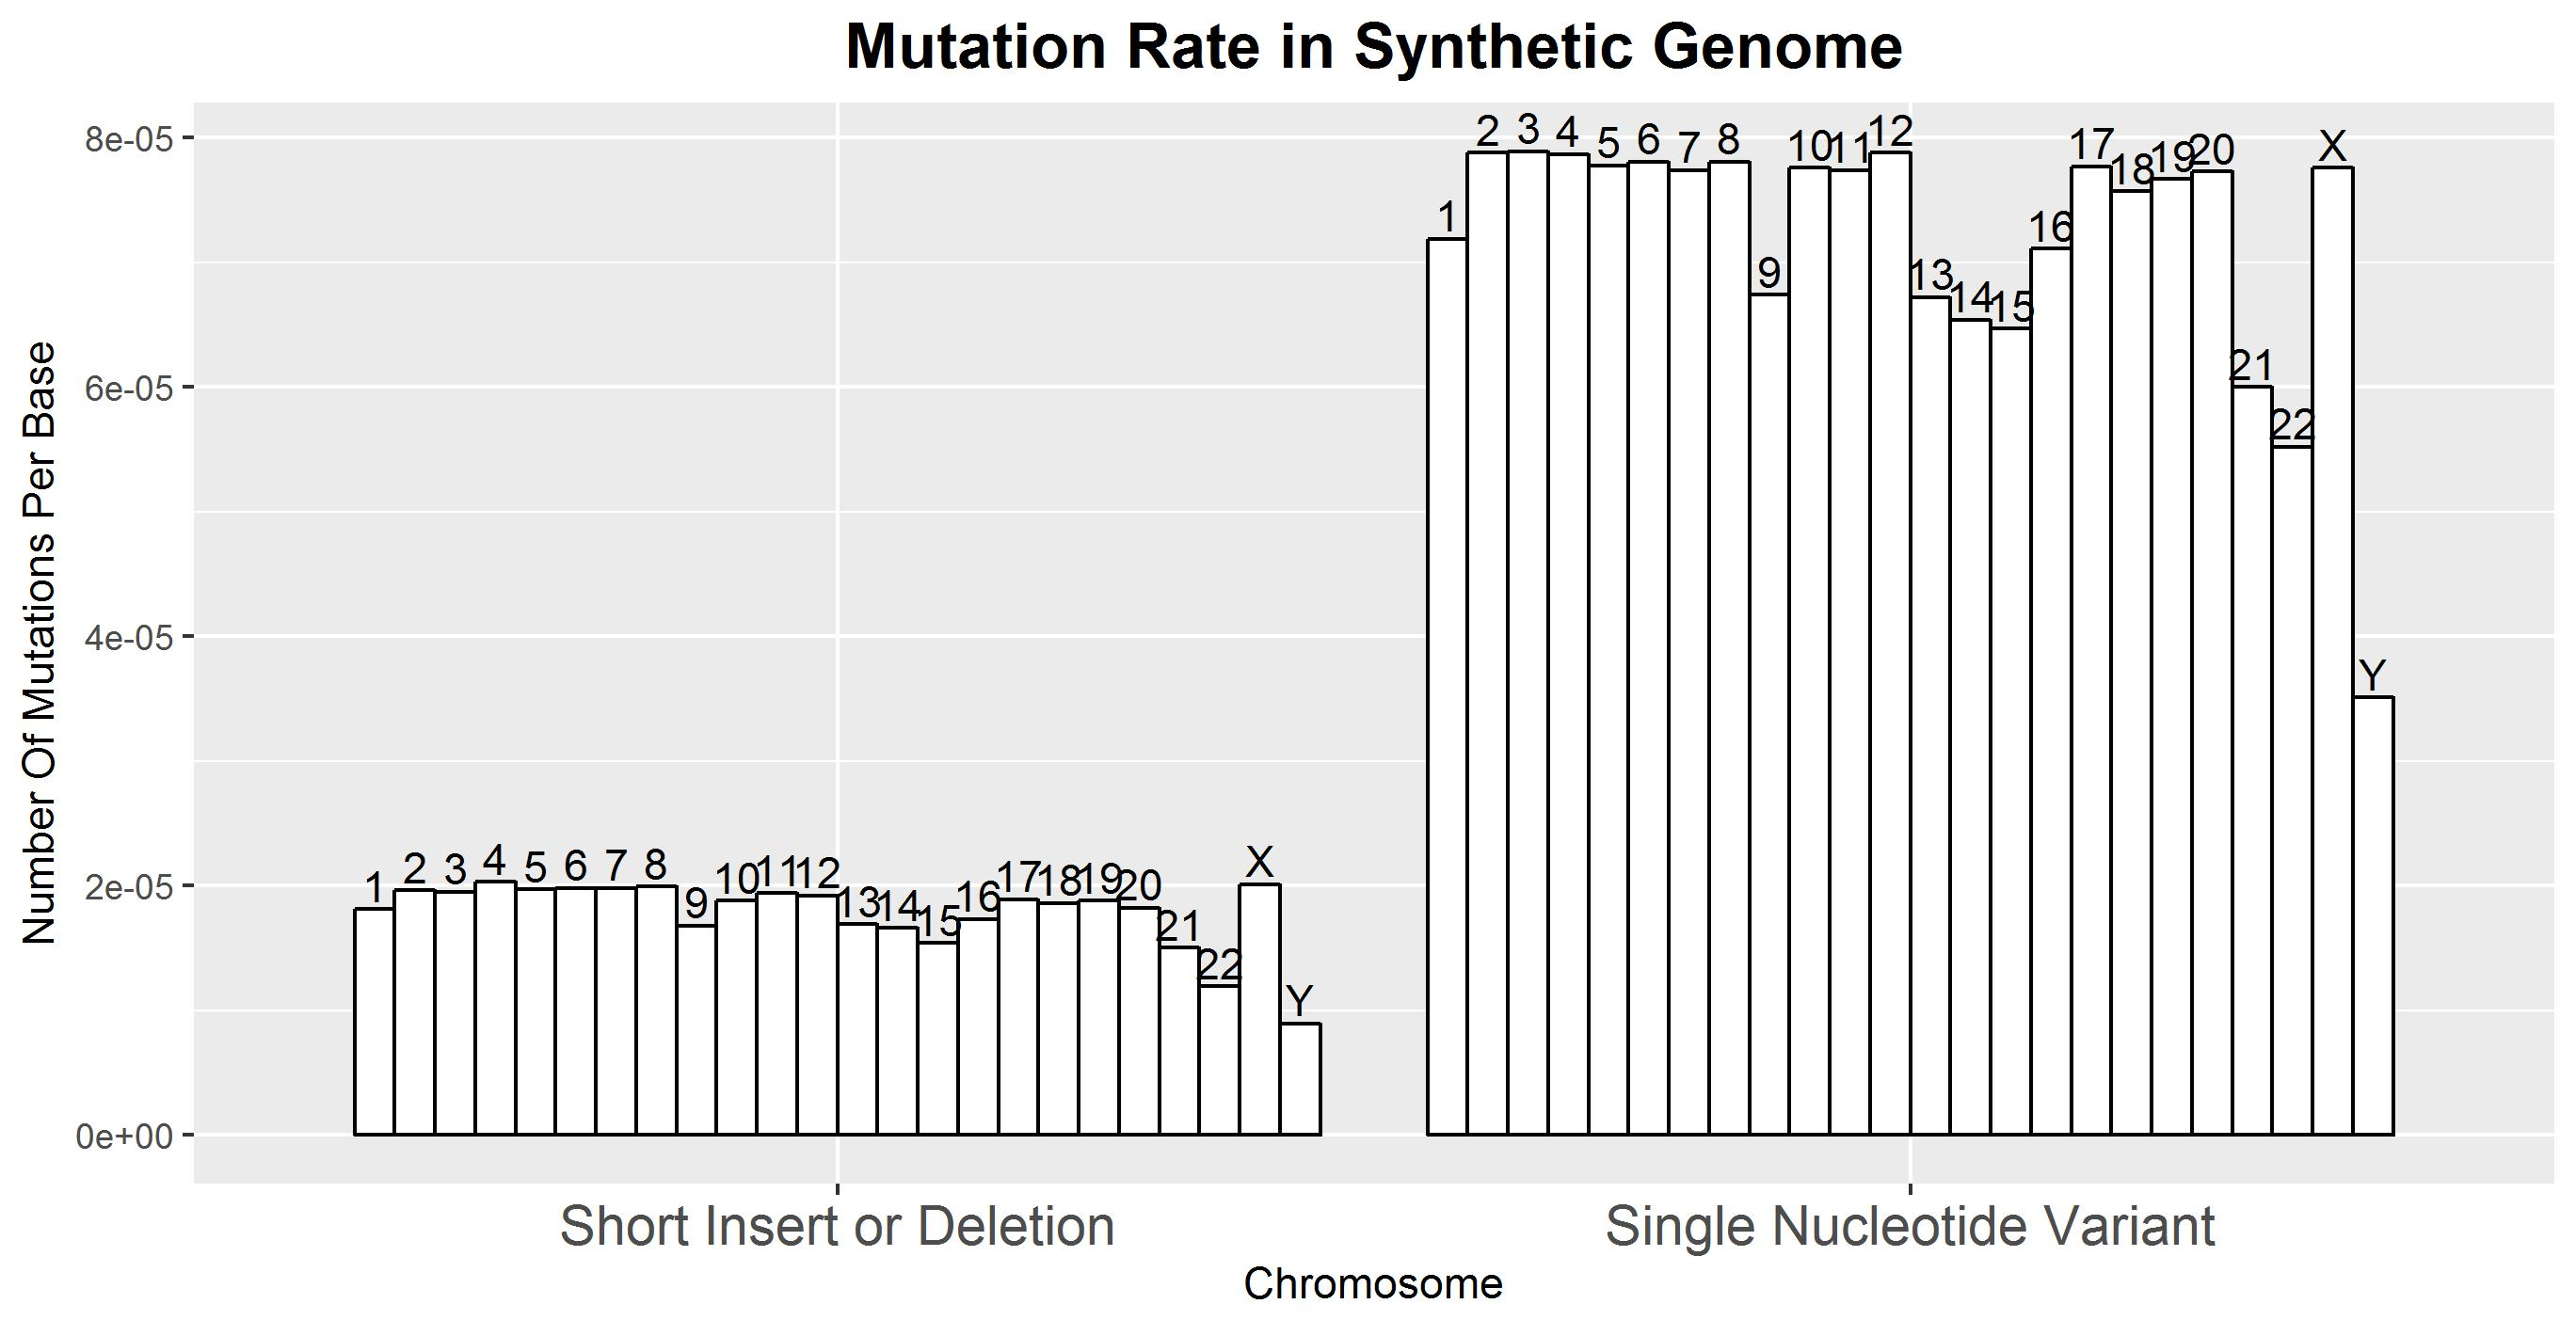
\includegraphics[width=\textwidth]{MutationRateInSimulatedGenome.jpg}
\centering
\end{figure}

\subsection{Network Architecture}
We systematically tested out various neural network architectures to see which architecture would perform the best. The architectures tested out were the flat architecture with 7 densely connected layers of 80 nodes each, the PCA + flat architecture which had the same neural network architecture, but before the input data was fed into the network a Principal Components Analysis was done to reduce the dataset to 8 principal components which was then used as input data for the neural network (please see Appendix A for more details of the PCA analysis). Finally, the last architecture we tested was the merged network. The overall structure of the networks can be seen in Figure N. \\\\

\begin{figure}[H]
\caption{Feature Engineering Table}
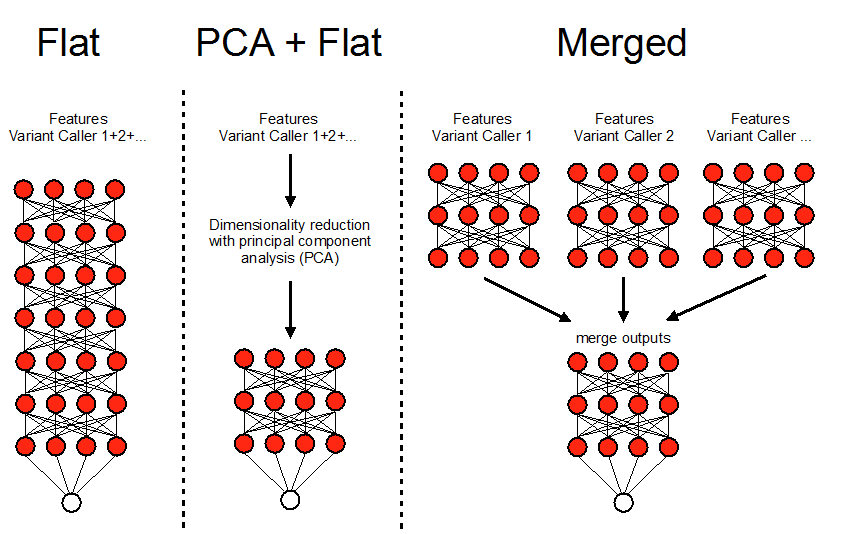
\includegraphics[width=\textwidth]{neuralnetworkstructure.png}
\centering
\end{figure}

\begin{figure}[H]
\caption{Feature Engineering Table}
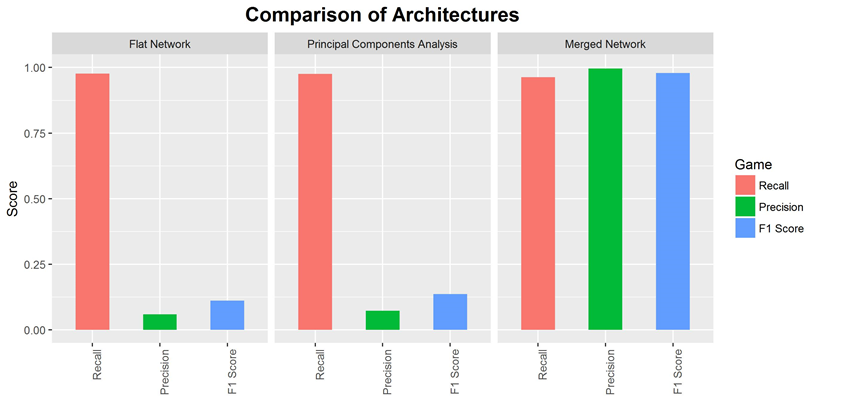
\includegraphics[width=\textwidth]{neuralnetworkstructureresults.png}
\centering
\end{figure}
Initially, with the flat network, the precision rate was very low, indicating that the neural network was unable to learn from the input feature set. We suspected that this was due to high dimensionality in the dataset, which led to our second architecture design, the PCA with flat analysis. Principal components analysis has been shown to be able to successfully improve learning in high dimensionality datasets (Chen et al., 2014; Van Der Maaten, Postma \& Van den Herik, 2009). Ultimately both failed to learn, indicating to us that perhaps the features from each of the callers had to be analysed separately before being passed into a separate neural network that did the final score computations. With this merged network, we managed to obtain a decent precision and F1 score that was far better than the previous two architectures. 


\subsection{Network Tuning and Optimisation}

A. Sample Balancing

In tuning our network, we sought to study how the various hyperparameters as well as the datastructure affected our network's ability to learn from the data. In particular, we focused on four issues, sample balancing, optimiser choise, learning rate choice and number of layers. These four issues are known to be critical in deep learning networks (CITATION x4). Our first concern was sample balancing - the simulated dataset contained an imbalance of positive training examples versus negative training examples. Such an sample imbalance has been known to affect learning adversely (Yan et al., 2015; López et al., 2012). Thus, we sought to study two methods of sample balancing, undersampling and oversampling. Our data was skewed with a high amount of negative training samples and  a low number of positive train samples. Thus, undersampling was implemented by removing negative training examples until the number of negative training examples was equal to the number of positive training examples. In oversampling, the Synthetic Minority Oversampling Technique(SMOTE) was done, which uses nearest neighbours to create more datapoints for the positive training example (see Appendix INSERT for more details). Figure 1 shows a representation of the normal, datasets on two principal components. Performance of all three methods 	


\begin{figure}[H]
\caption{Feature Engineering Table}
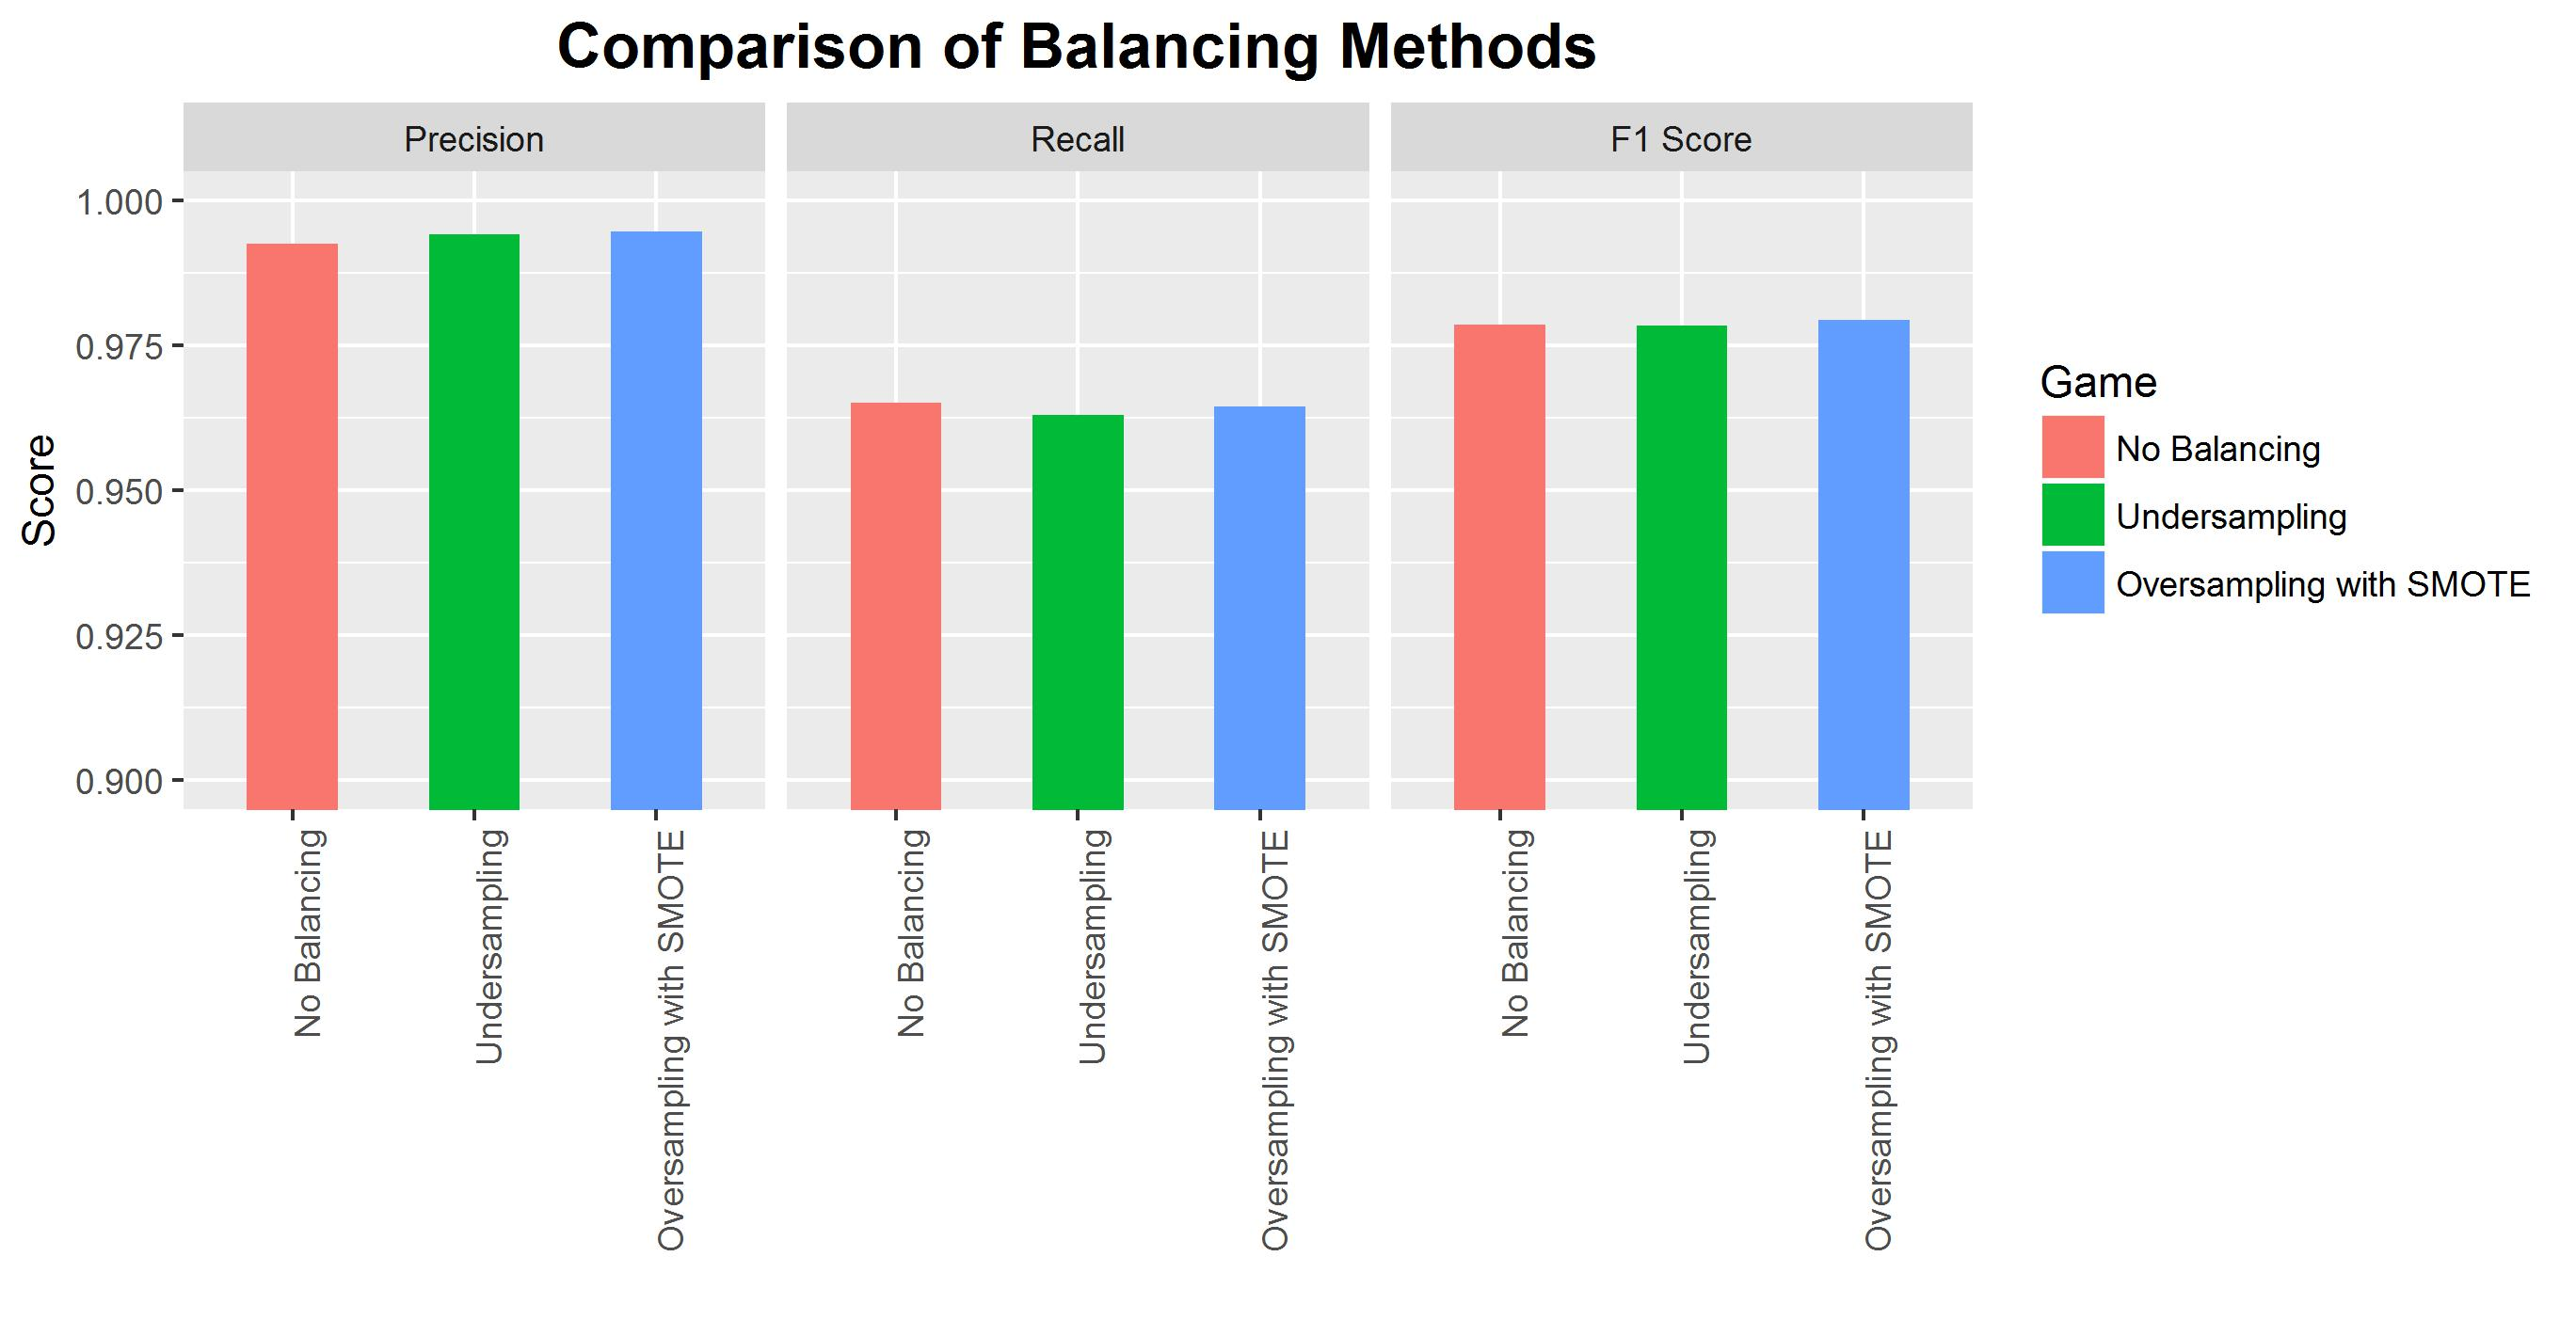
\includegraphics[width=\textwidth]{comparisonofbalancingmethods.png}
\centering
\end{figure}

B. Optimiser and Learning Rates
Optimisers have also been well studied and known to be important in neural network training (CITATION). Optimiser choice is critical as the optimisers determine how the weights and gradients are updated in the network, thus playing an integral part in learning. We studied 3 well-known optimisers for use in our network, ADAM, RMSprop and Stocastic Gradient Descent. ADAM is an adaptive learning rate optimiser that stores . is known to be validated for dataset, and is an improvement. RMS-prop is another adaptive learning rate optimiser that stores is an unpublished dataset, but has been known to work well for experimental learning datasets. Stocastic gradient descent is the simplest learning model with no adaptive learning rate, but is a useful model because it is the easiest to understand mathematically. For more information on the mathematical foundations of each optimiser, please see Appendix N. For the three optimisers, we ran tests to study the accuracy of the neural network running on each optimisers to predict true variants (Figure N).

\begin{figure}[H]
\caption{Feature Engineering Table}
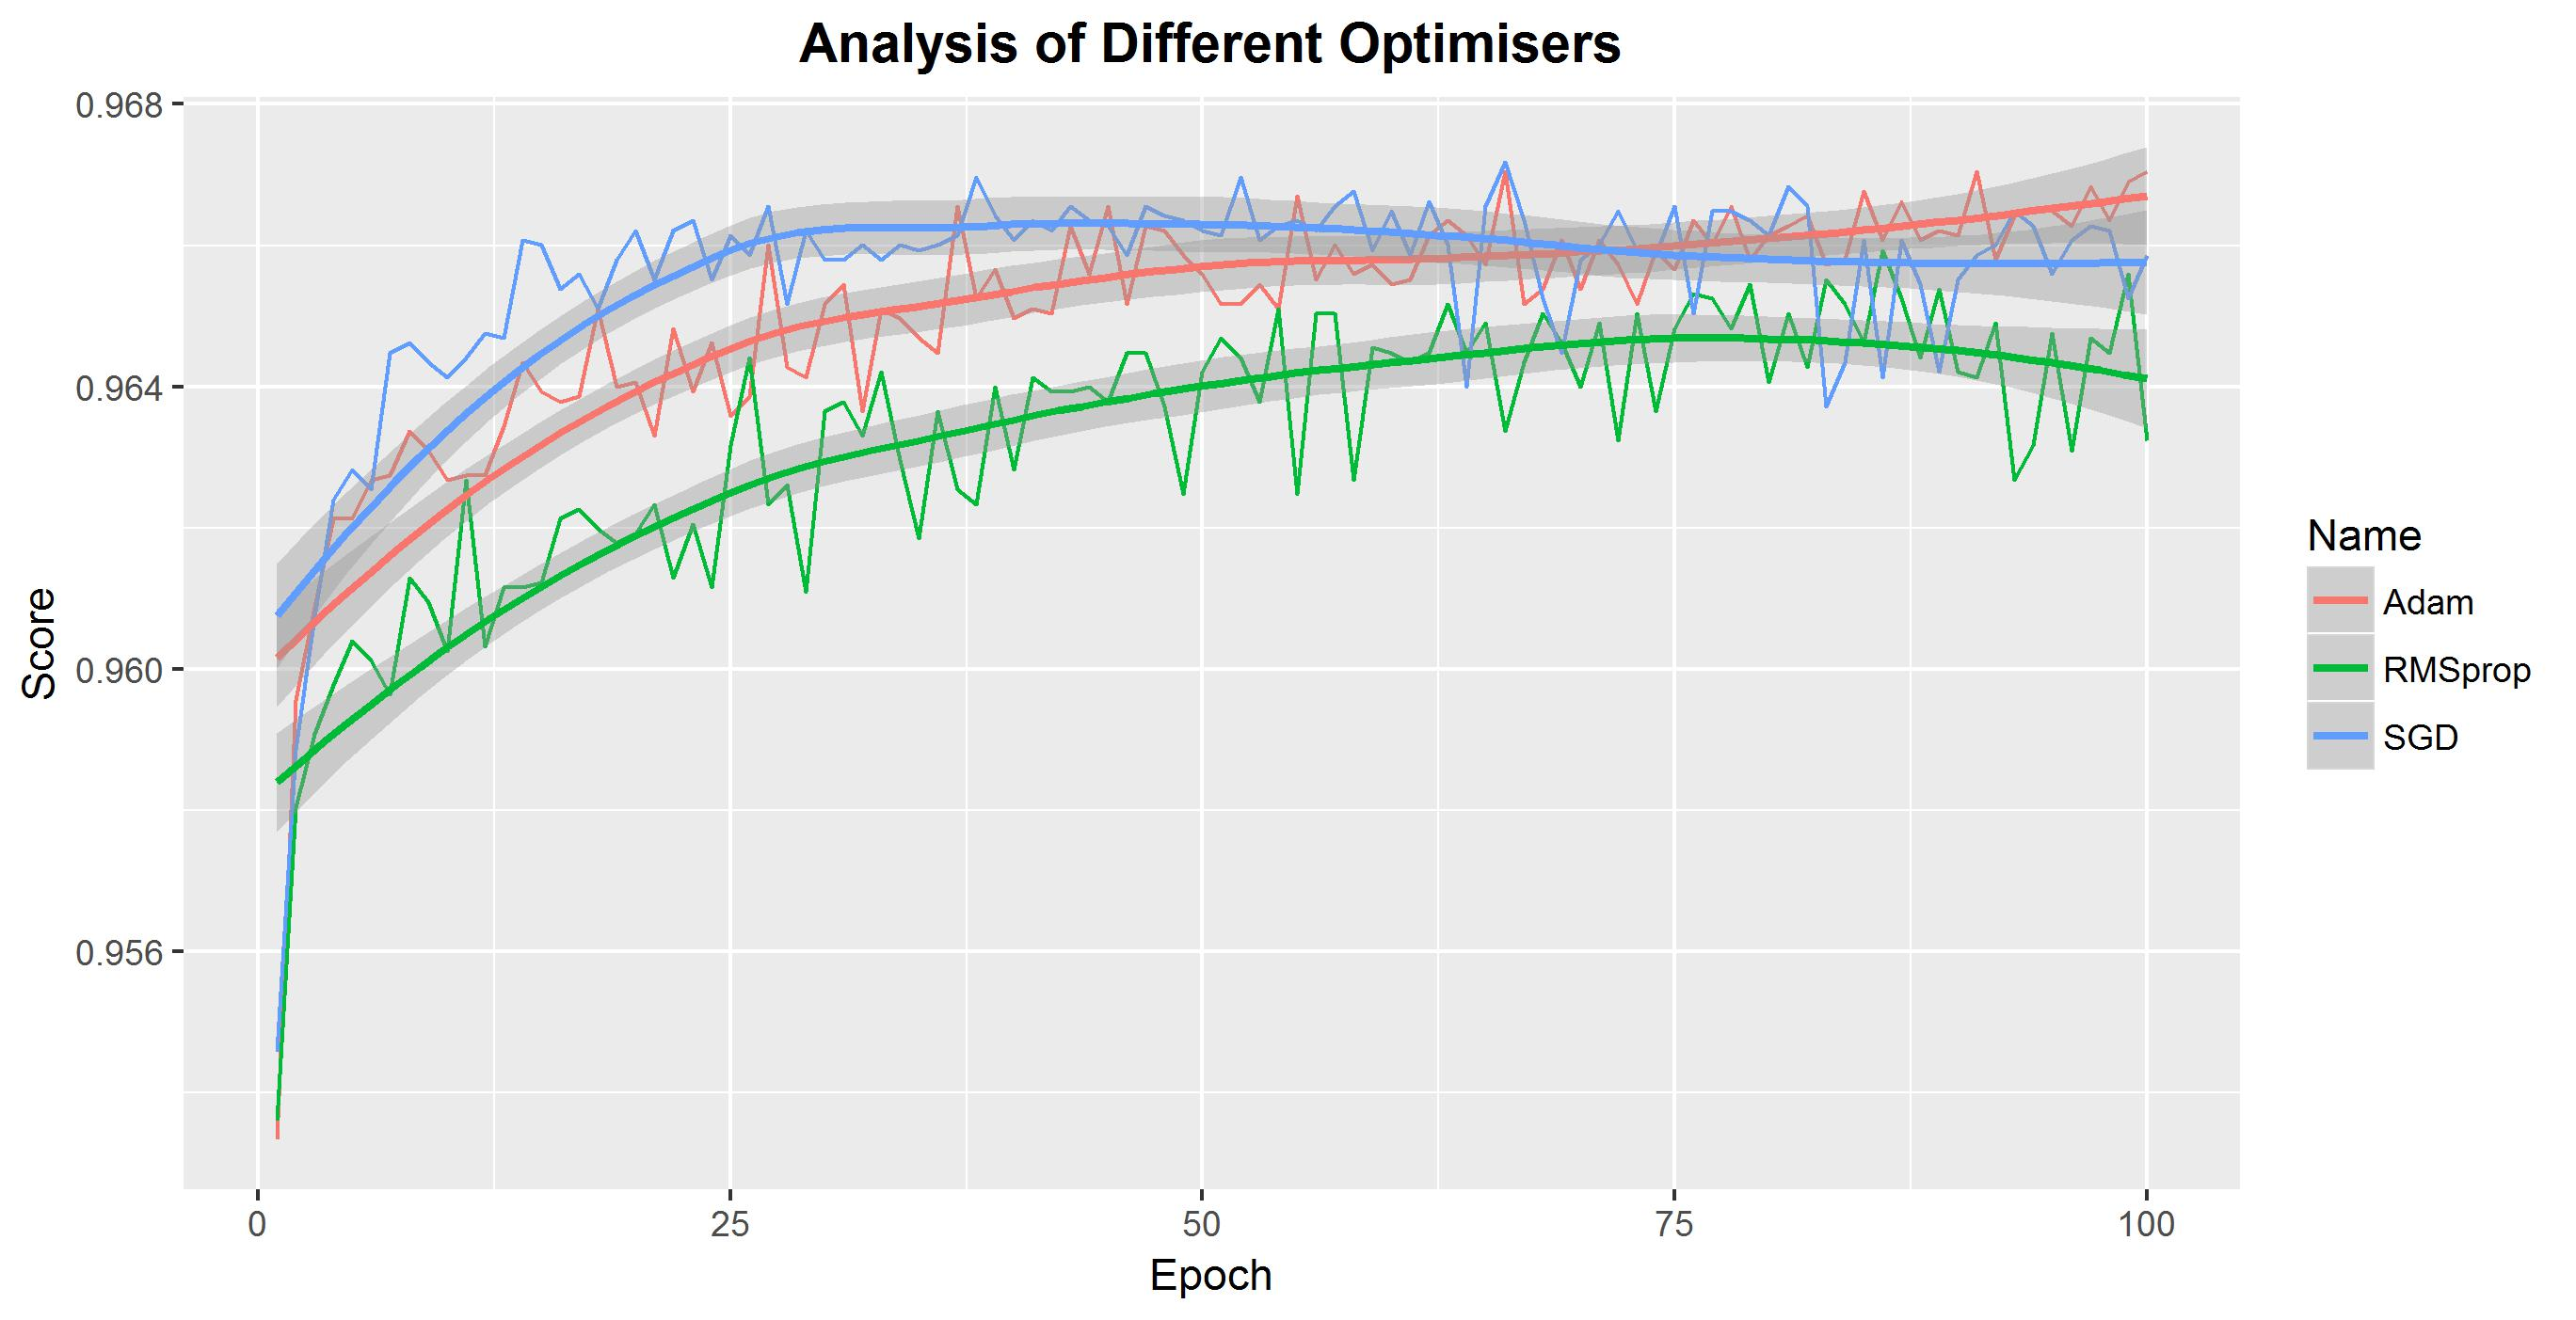
\includegraphics[width=\textwidth]{optimiserlearning.jpg}
\centering
\end{figure}

ADAM was noted to plateau at an accuracy at X epochs. This was higher than RMSprop at N after 100 epochs and SGD at Y after 100 epochs. This indicates that ADAM seems to be the most suitable learning rate method. Furthermore, we note a stable learning curve for ADAM, indicating it is able to learn and update the gradients in the neural network to learn from input data. Interestingly, we note some chaotic behaviour for ADAM after it has hit plateau, bouncing up and down in terms. This could be due to a minimum finding problem where it has already found the minimum and so every gradient moves it away from the minimum causing it to decrease, and then it goes back to the minimum again. Such behaviour has been noted in X. This is known to be not an issue with the algorithm but more of due to the fact that it has already found the minimum. Thus, we decided to use ADAM as our optimiser. We also looked at various learning rate for Adam (Figure N), and found that the most stable learning could be found at LR = 0.00001. Thus, we chose this to be our learning rate.


\begin{figure}[H]
\caption{Feature Engineering Table}
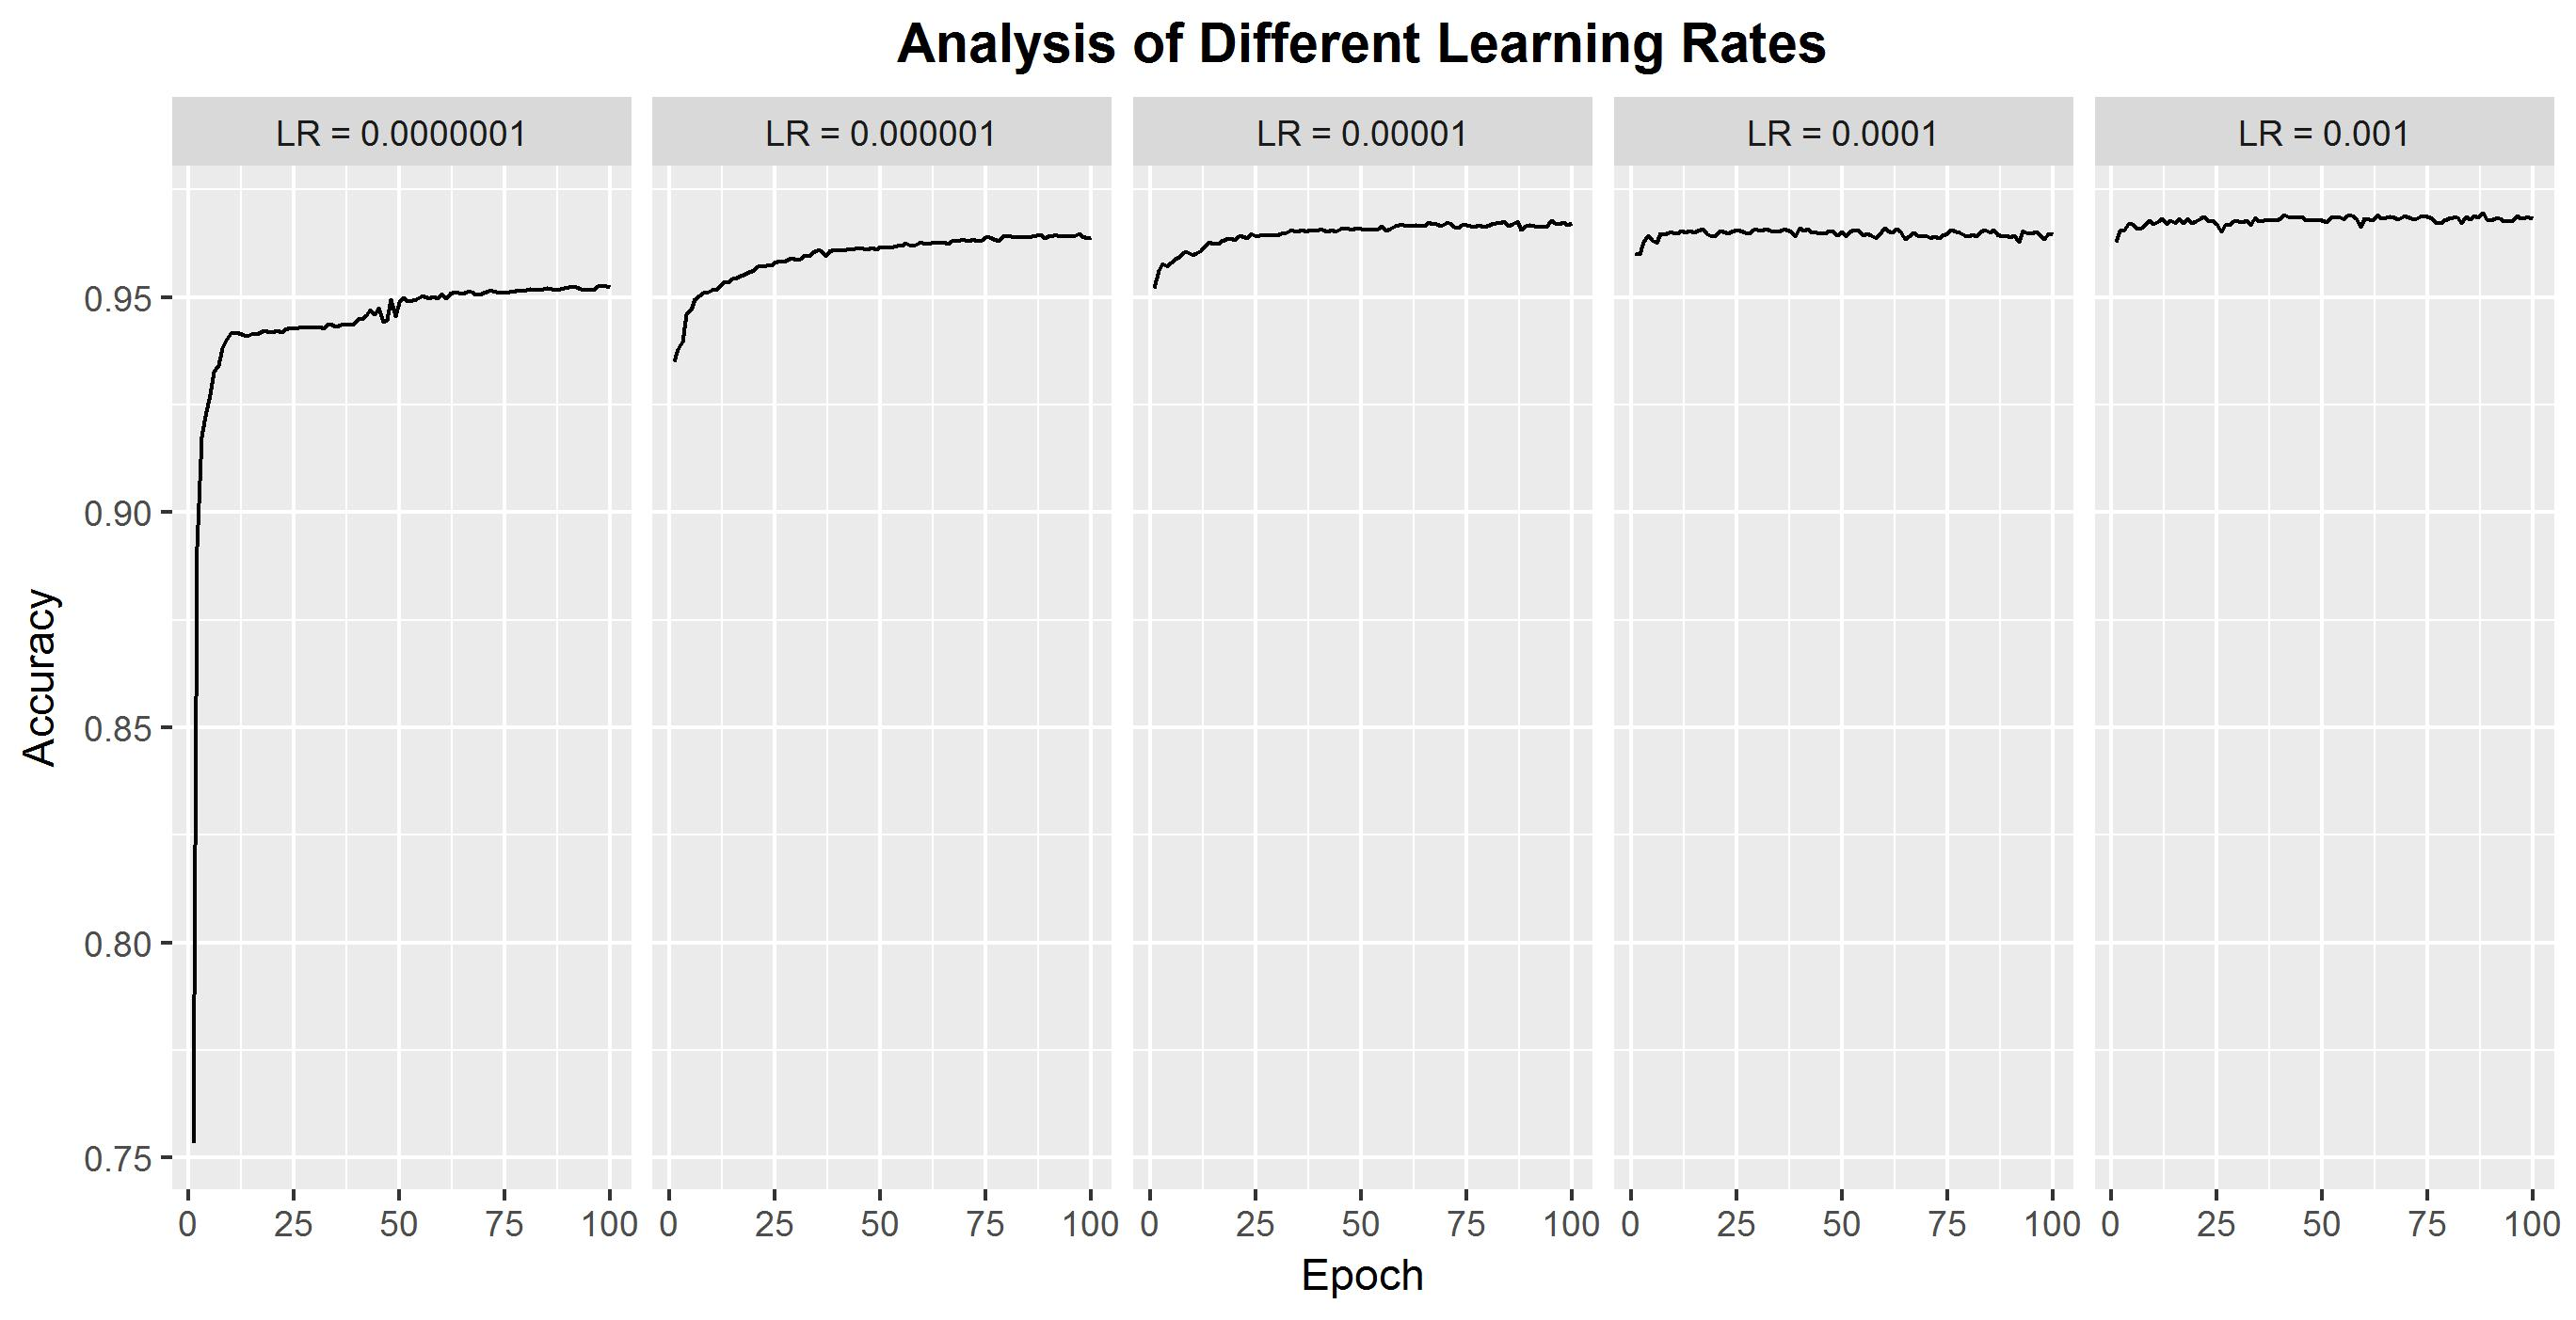
\includegraphics[width=\textwidth]{learningrates.jpg}
\centering
\end{figure}


C. Number of Layers 
Finally, we studied how many layers should be in the neural network. The number of layers is critical as it determines what kind of information and the representation of data that can be captured by the neural network. We studied 4 different neural network structures (4 layers to 7 layers). 

\begin{figure}[H]
\caption{Feature Engineering Table}
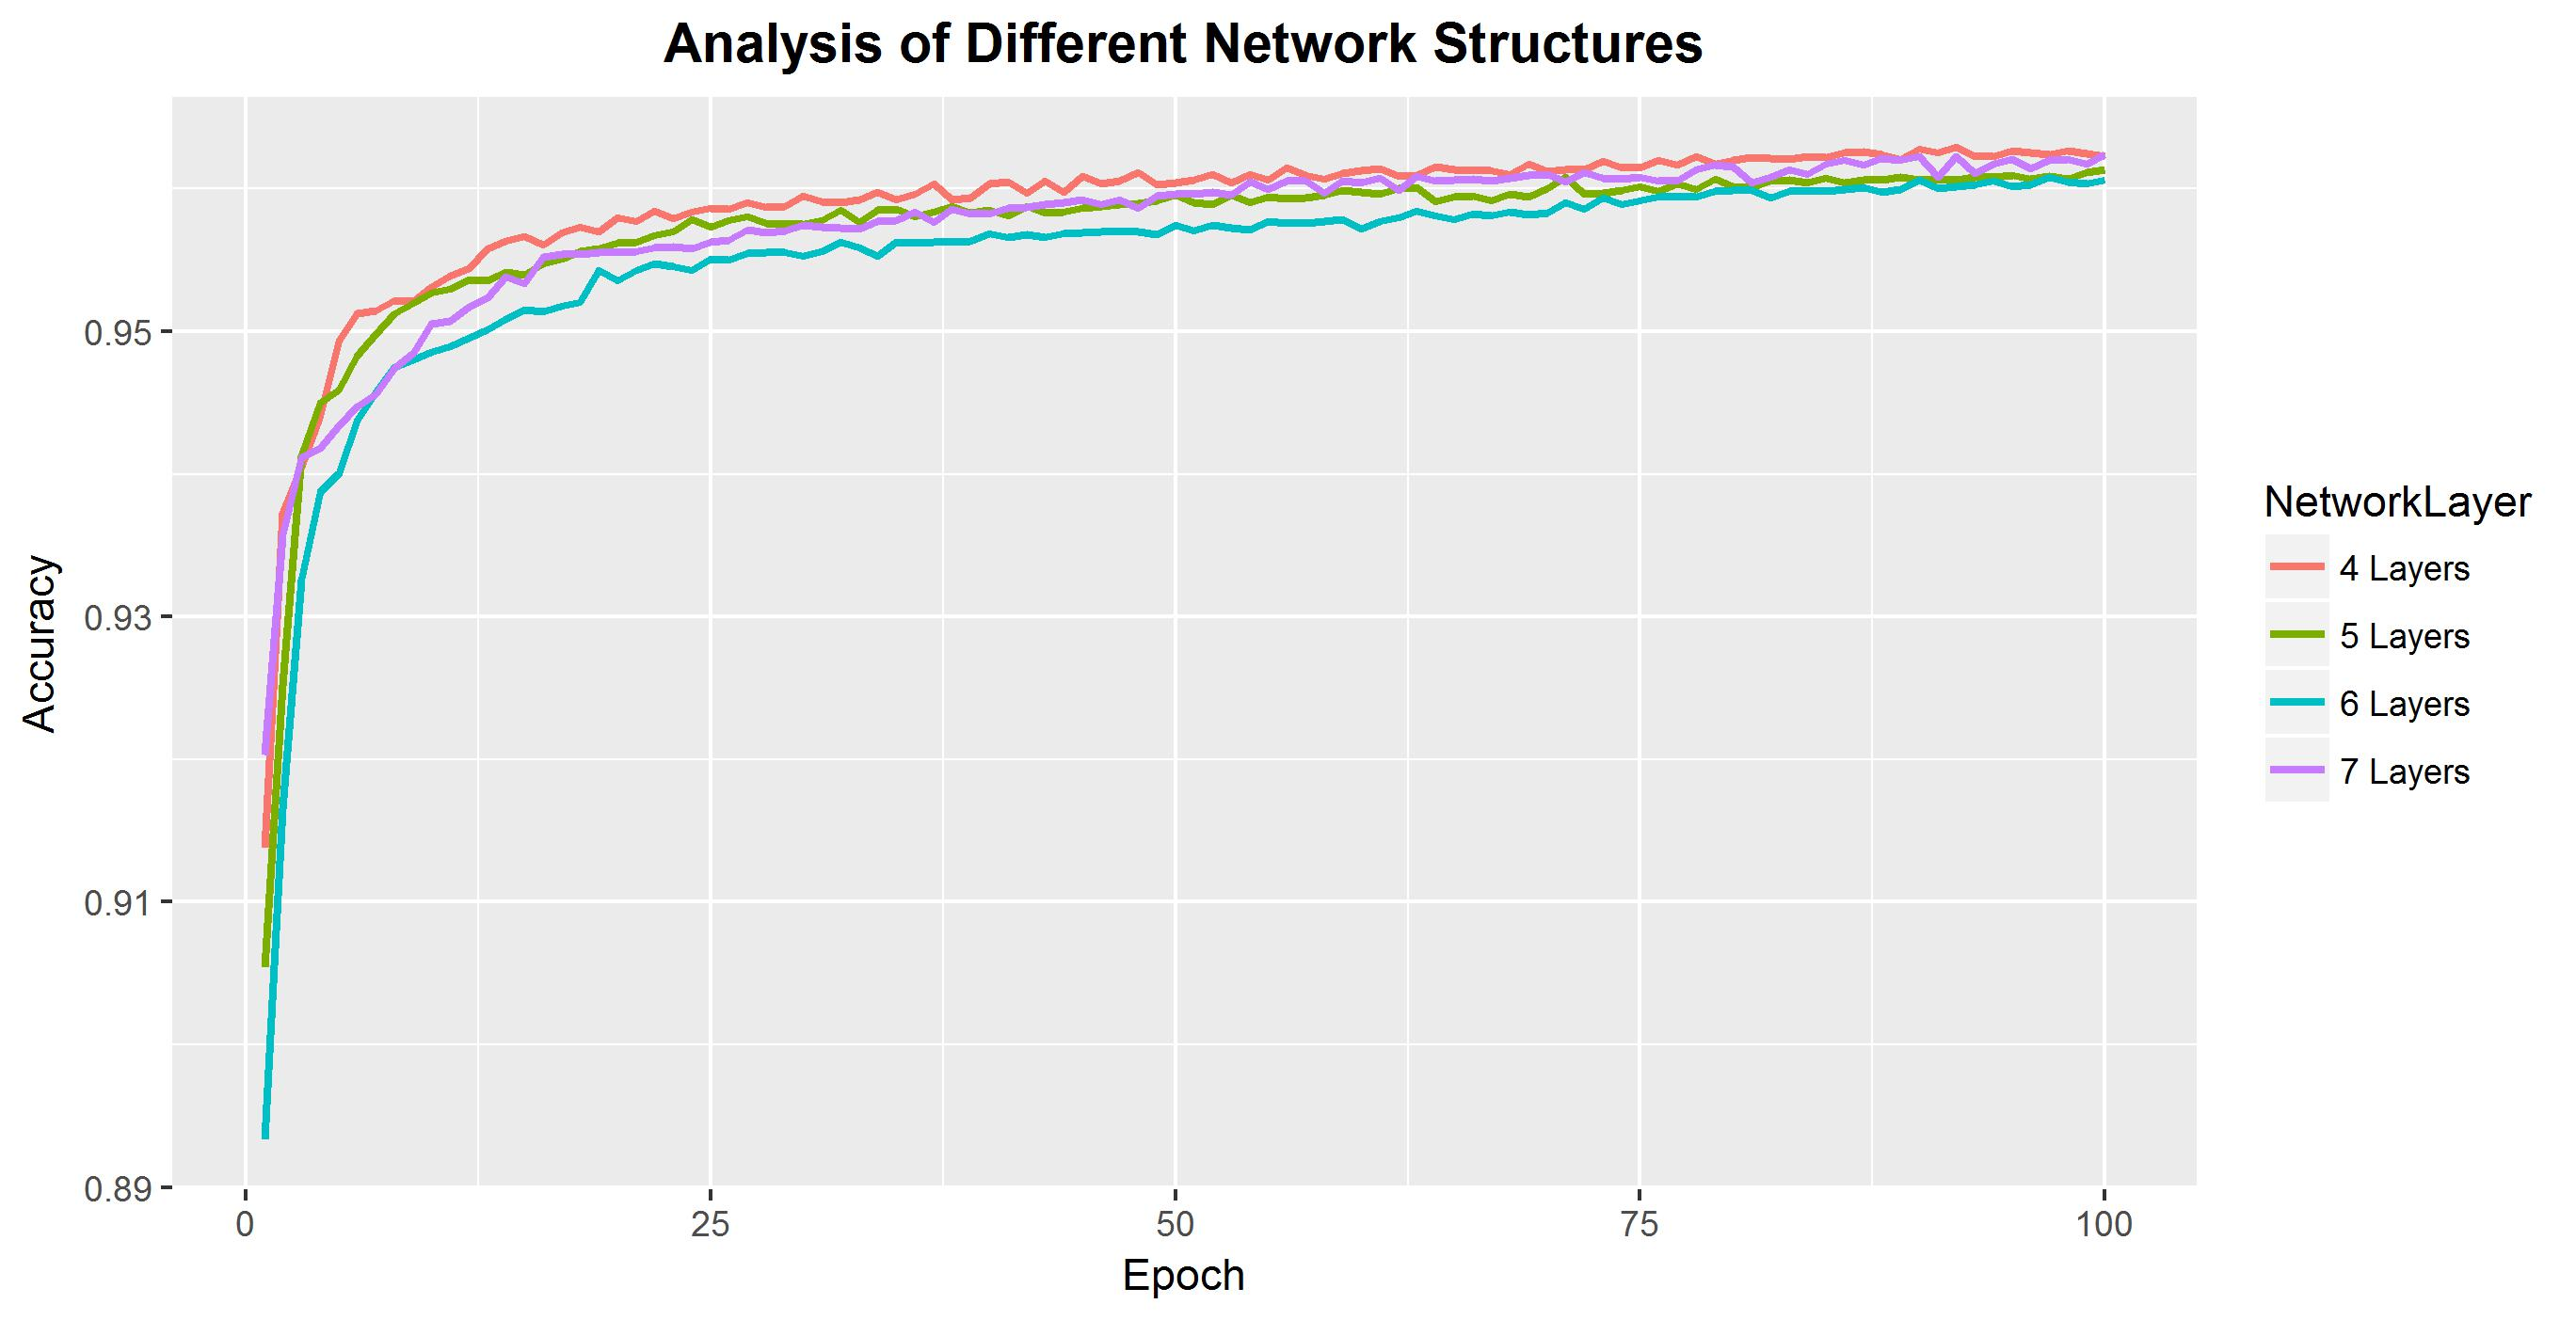
\includegraphics[width=\textwidth]{networkstructure.jpg}
\centering
\end{figure}

From analysing the accuracies of the different layers, we find that 4 layers and 7 layers networks seem the best at learning from the input data. We decided on the 7 layer network as it seemed best able to learn from the input dataset. The final network was decided in the structure below - 

\begin{figure}[H]
\caption{Feature Engineering Table}
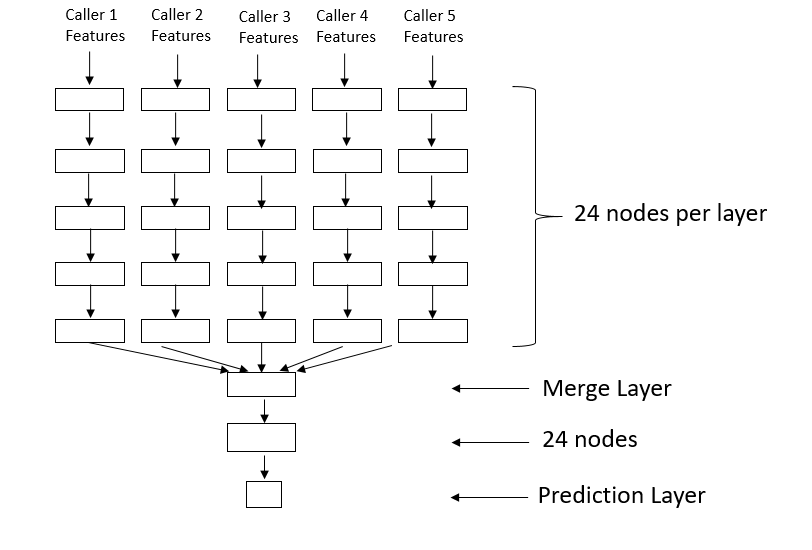
\includegraphics[width=\textwidth]{neuralnetworkarchitecturefinal.png}
\centering
\end{figure}



\subsection{Benchmarking of Network with Mason Datasets}
From optimisation steps, we finalised the network architecture as seen in figure 1. We choose the learning rate to be 0.00003, and the optimiser used was Adam. With this network, we benchmarked the neural network against the single variant callers, as well as concordance callers, which are an integration of the outputs of the 5 variant callers. Specifically, the n-concordance variant callers are defined as the set of calls that any n callers agree upon - so 1-concordance includes all the calls made by all callers and 4-concordance includes all the calls made by any 4 callers. Concordance calling using an ensemble of callers has been shown to be an improvement over using single variant callers (CITATION). 

\begin{figure}[H]
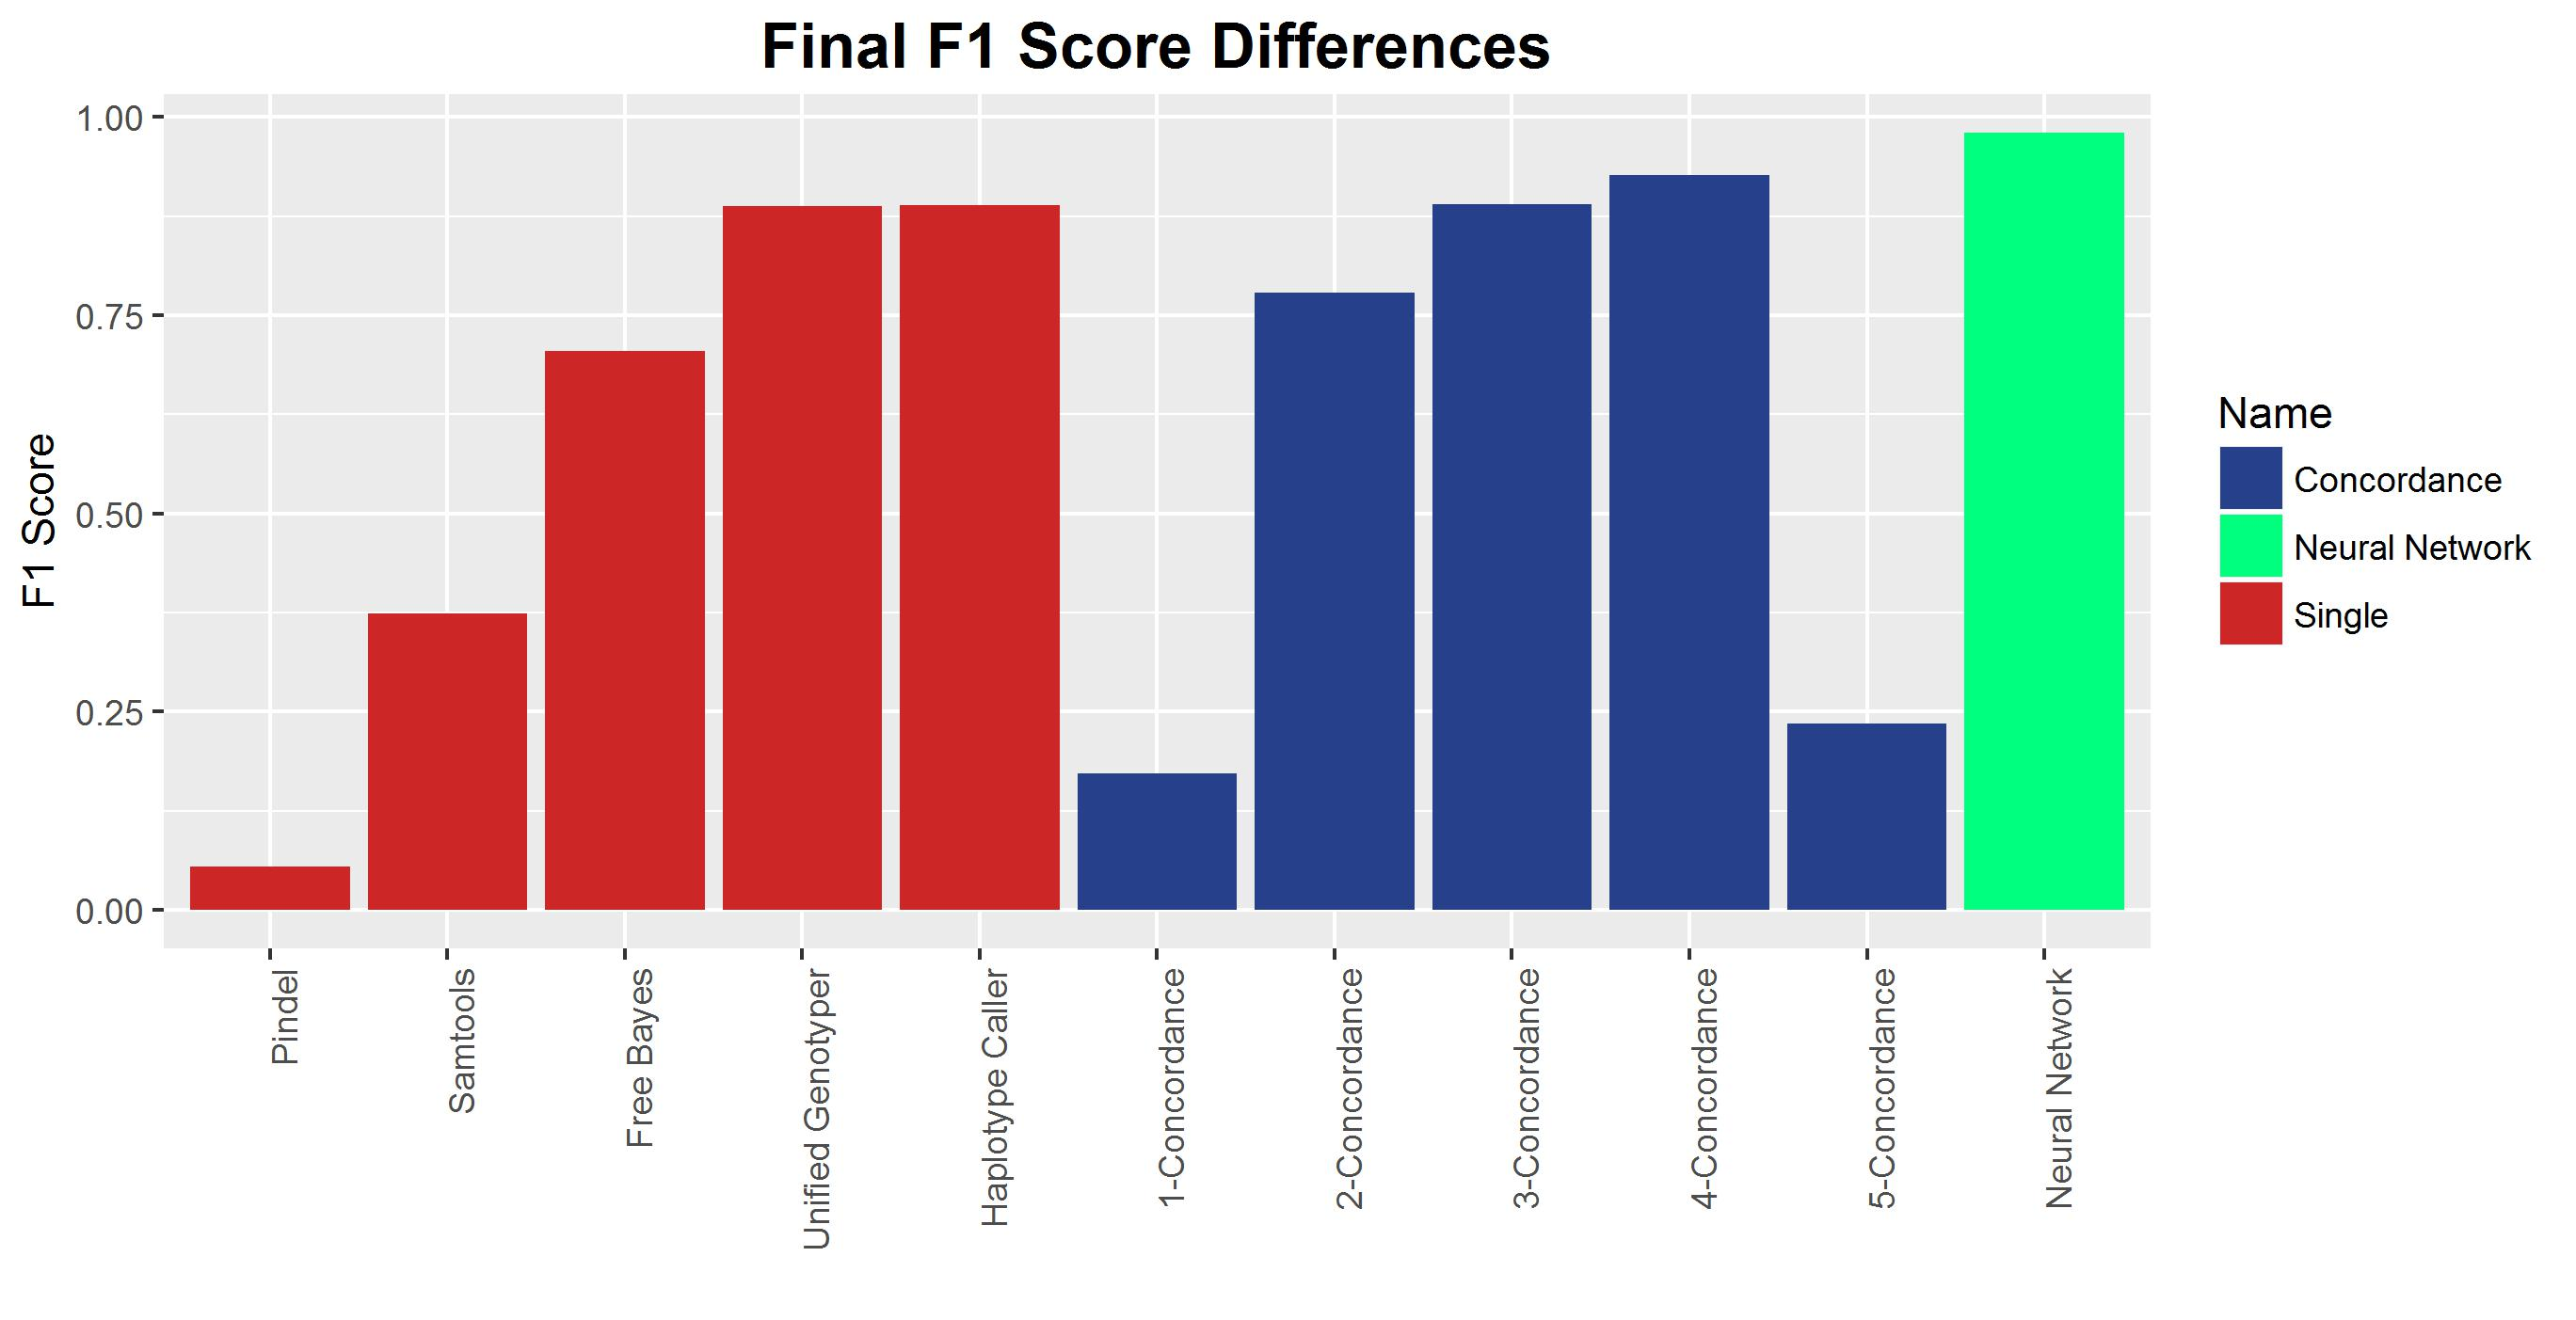
\includegraphics[width=\textwidth]{final_f1scores_results_all.jpg}
\caption{Comparison of Variant Callers}
\centering
\end{figure}

In terms of overall F1 score, we see that the neural network was able to outperform single and concordance-based callers. This provides strong evidence that the neural network is able to learn from the input features whether the variant call is real or not, validating its usage in variant calling. Looking at the exact precision, recall and F1 scores of the top 2 variant callers as well as the best single variant caller versus the neural network, we find that the neural network is more precise than both, but the recall is rather similar. This indicates the neural network is able to sieve out the false positives inside best calling methods. 

\begin{figure}[H]
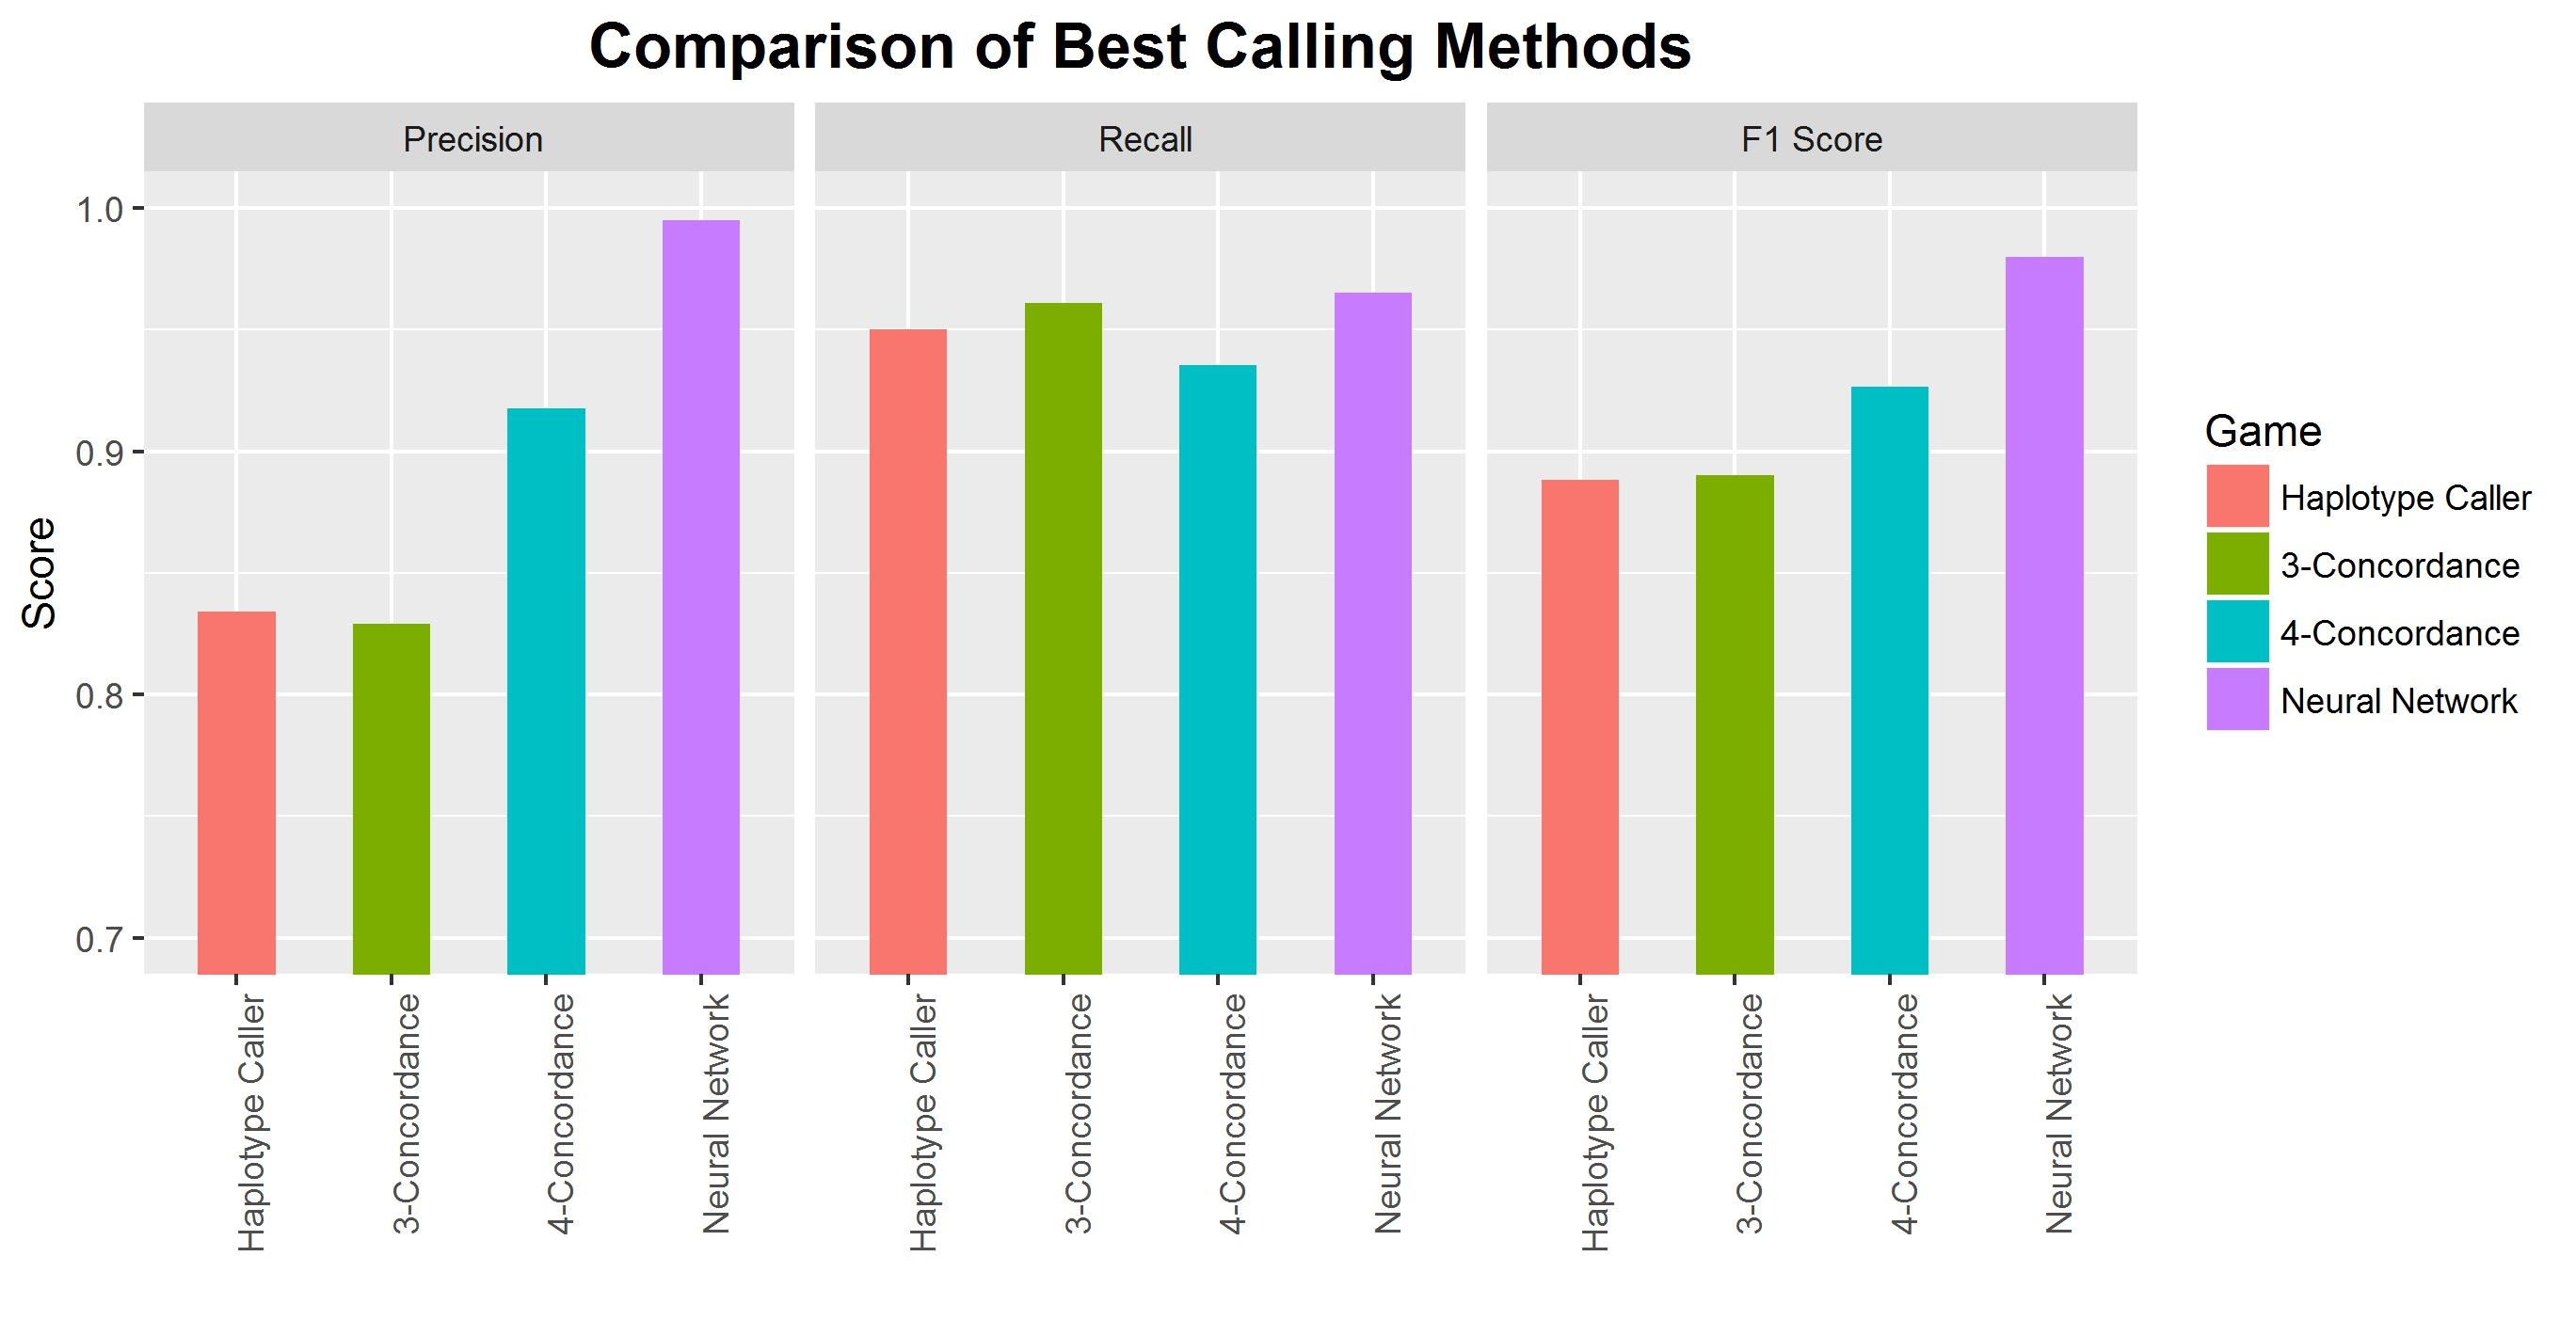
\includegraphics[width=\textwidth]{masonheadsupcomparison.jpg}
\caption{Comparison of Variant Callers}
\centering
\end{figure}

Further evidence of the ability of the neural networks to learn comes from basic principal components analysis of the datasets. 

\subsection{Benchmarking of Network with NA Datasets}
After verification of the neural network architecture, optimised parameters and ability to learn with a simulated dataset, we sought to analyse a real dataset to set the validity of the neural network in validating variants. We studied the NA12878 Genome In a Bottle dataset (CITATION), which has been used in other variant calling validation pipelines(CITATION) and contains a set of high confidence variant calls which we can use as ground truth for training and validation. This set of high confidence variant calls are obtained from multiple iterations of orthogonal sequencing methods (using Solid, Illumina platforms, Roche 454 sequencing and Ion torrent technologies). The usage of multiple platforms enables an intersection of variants that can be considered as the ground truth. We then sought to see if our neural network can predict the ground truth better than single or concordance based variant callers. We applied the same methodology to the sequences as with the simulated data and then used our neural network to predict the true variants. As can be seen from the figure, the neural network was able to predict with higher precision the best single caller, haplotype caller and the 2 best concordance callers, 3-concordance and 4-concordance. In terms of recall, the recall rates were the same between Haplotype Caller, 3 concordance and the neural network. This was an interesting observation as it shows that the neural network is more aggressive in making calls than the 4 concordance neural network, and it is more likely that the calls it makes are correct. Ultimately when we looked at the f1 score, the neural network was able to outperform these variant callers. This validates our neural network pipeline and indicates that we are able to learn from the input features. 

\begin{figure}[H]
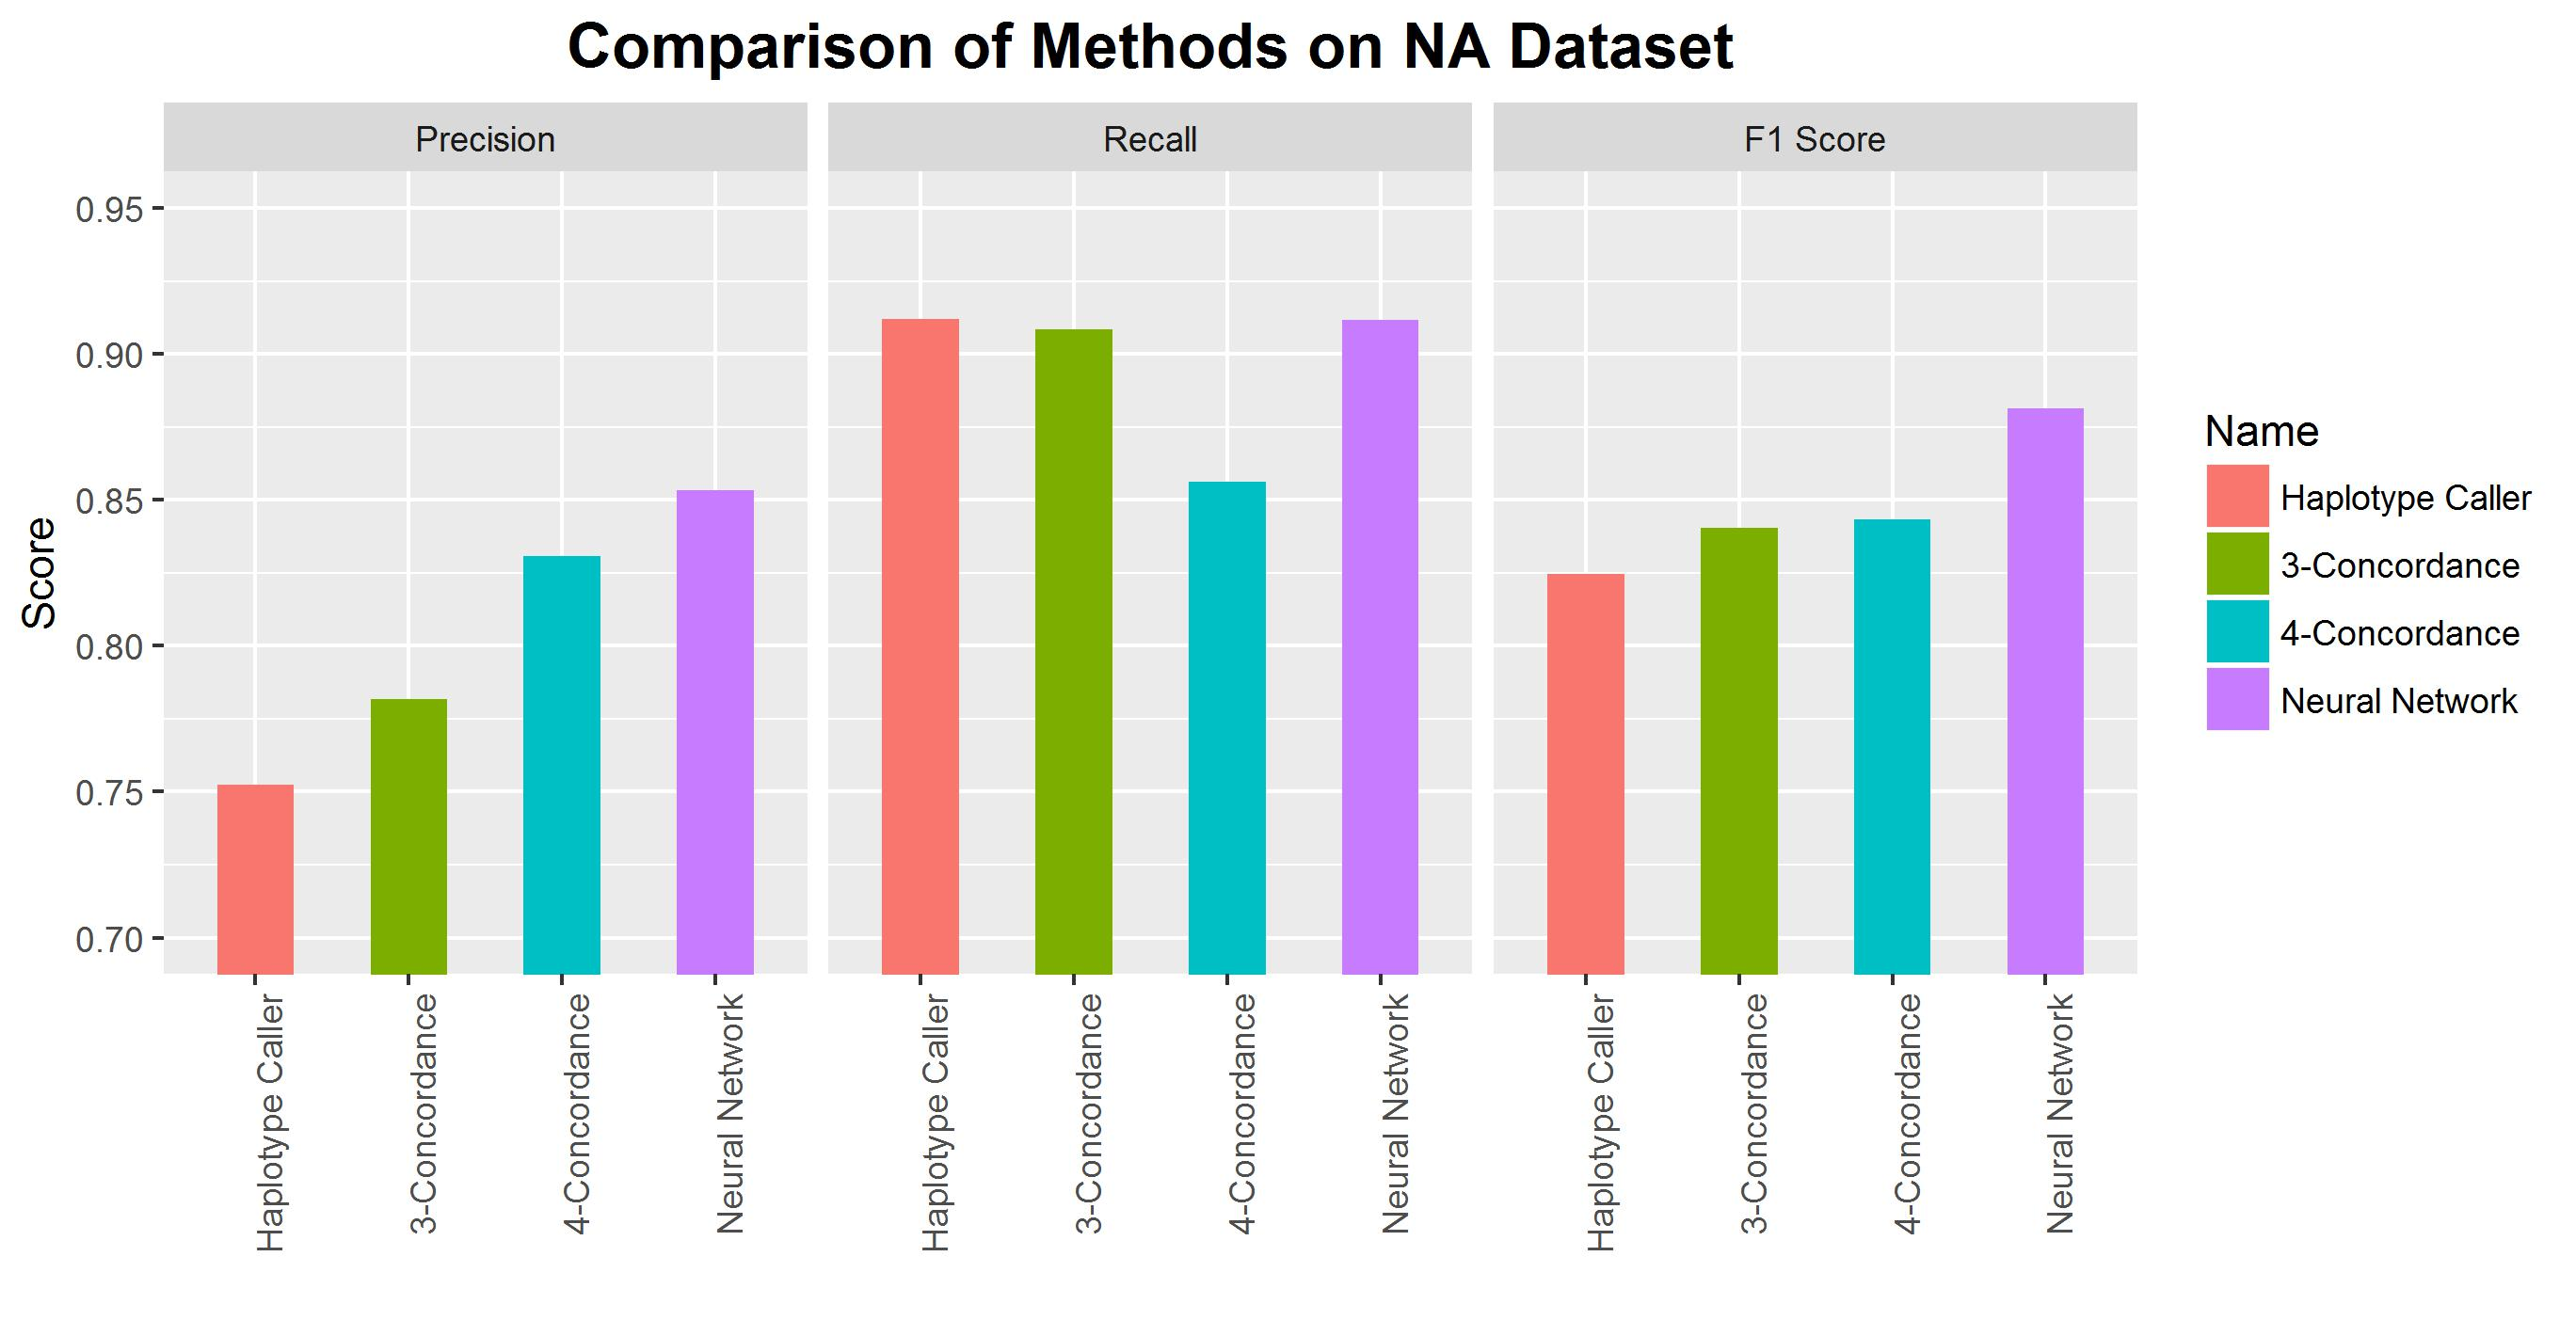
\includegraphics[width=\textwidth]{naheadsupcomparison.jpg}
\caption{Comparison of Variant Callers}
\centering
\end{figure}

\subsection{Analysis of gene importance using Bayesian Ranking systems}
After validation of high confidence calls, we sought to enable a clear and understandable ranking of genes. We first build a Bayesian network analysis using known functional annotations from AnnoVar. These were subsequently used to compute the Bayesian probability ranking, which is shown in Figure N below.


\begin{figure}[H]
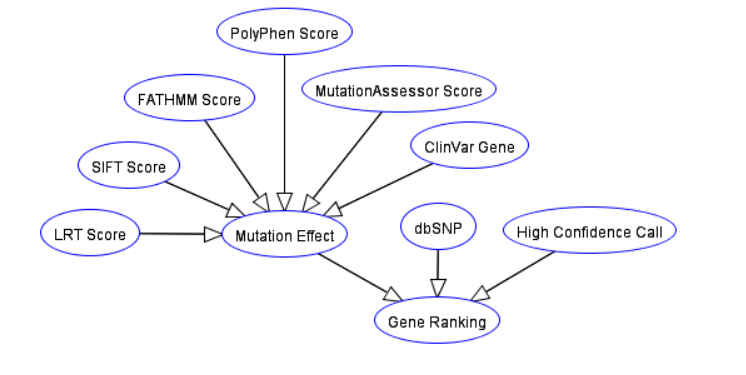
\includegraphics[width=\textwidth]{bayesiannetwork.png}
\caption{Comparison of Variant Callers}
\centering
\end{figure}

This network structure was chosen as we wanted to use three different sets of information to update the probability of the gene being important. Firstly, the confidence of the call should matter in how important it is - the more likely a gene is real, the more important it should be. Secondly, the rank should also be determined by how common the variation is, based on studying known SNP polymorphism rates. If it is a common SNP, then the ranking should be downgraded as it is less likely to be a driver mutation. Finally, we sought to predict the overall effect of mutations via an ensemble of mutation effect predictors. These predictors use different methods to predict the average effect of that mutation - based on statistical methods like position specific substitution matrixes and Hidden Markov Models to study the effect of a mutation on protein structure and function. We also used the ClinVar database, a curated repository of known Human variants and their resulting phenotypes. These scores were then aggregated to update the probability of the mutation effect.

\begin{figure}[H]
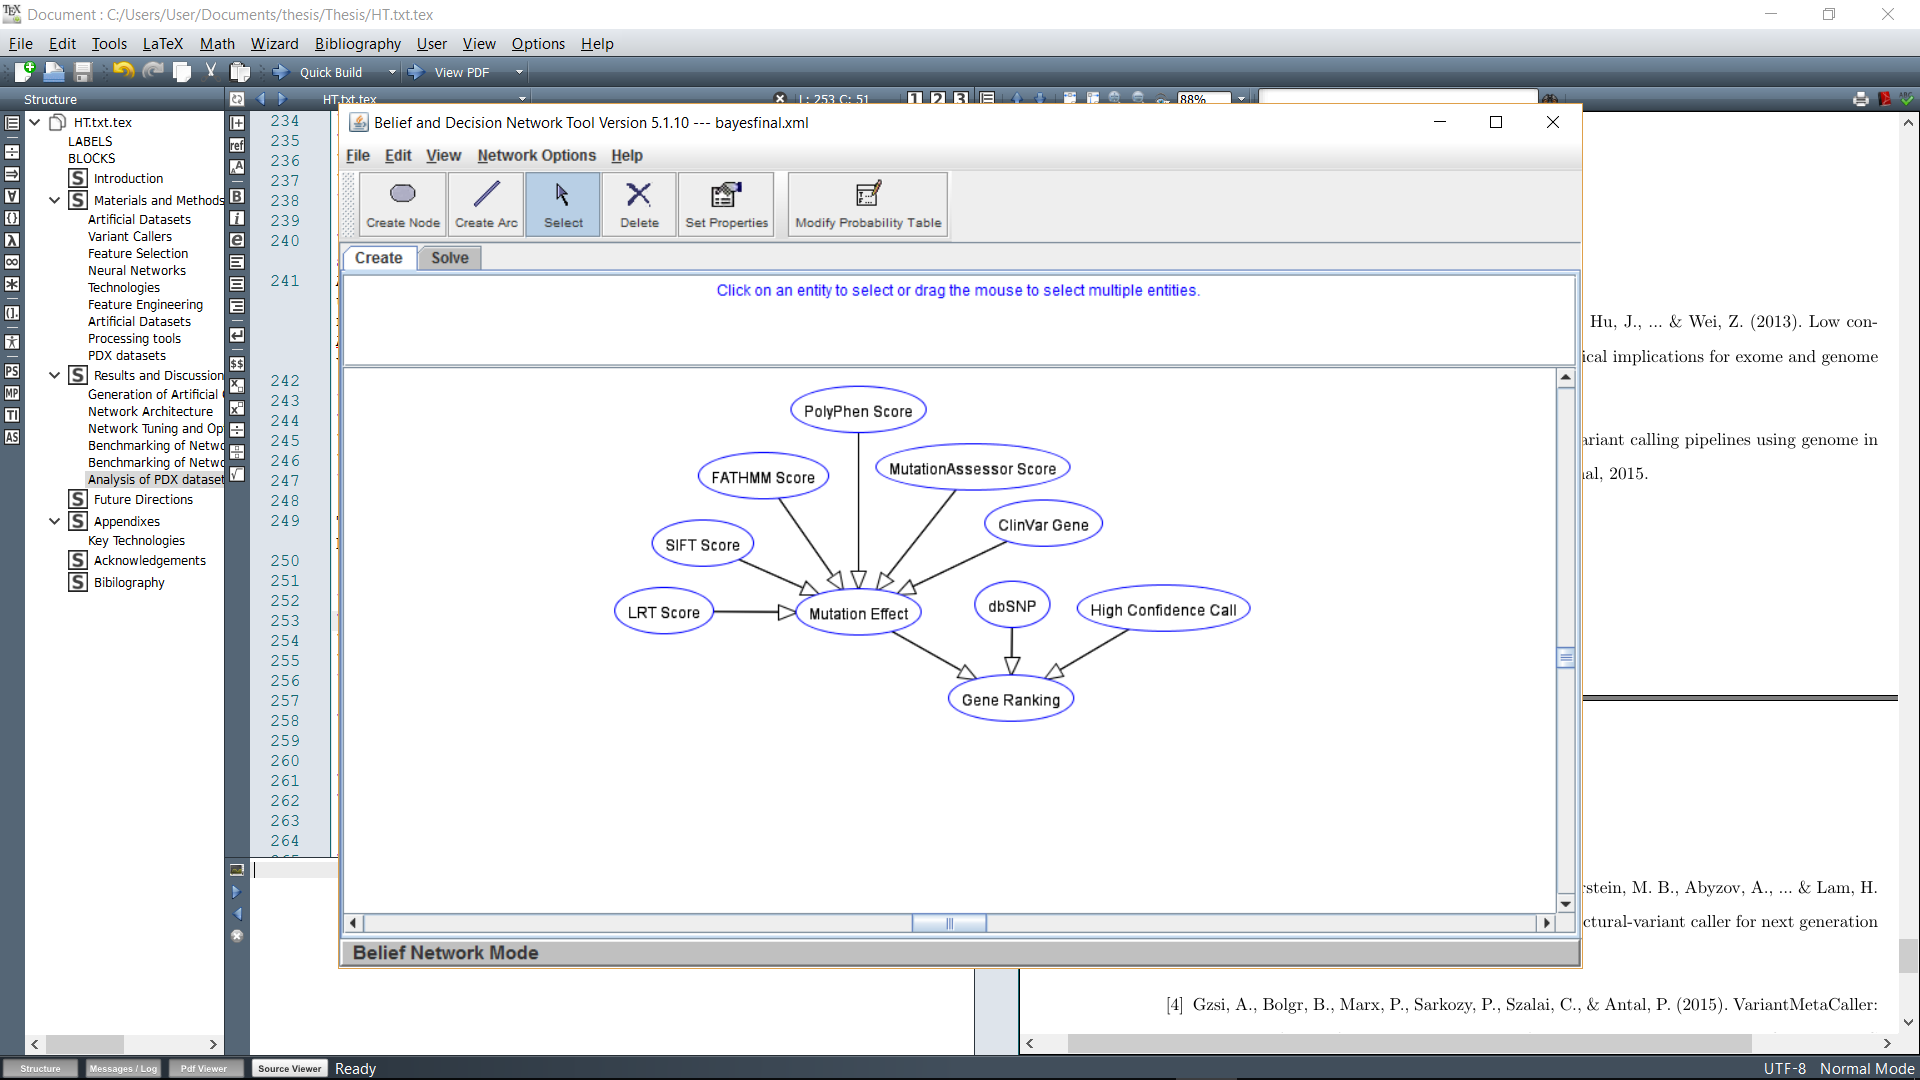
\includegraphics[width=\textwidth]{annovarfeatures.png}
\caption{Comparison of Variant Callers}
\centering
\end{figure}


Based on scores provided, we report the update the conditional probabilities using the probabilities chain rule - for the first level, this is given as \\
\begin{equation}
\begin{split}
P(Impt | (Del  \ \cap \ Uncom  \cap High\ Conc)) =  \ \ P(&Impt \cap Del  \ \cap \ Uncom \cap High \ Conc ) \\ \ * \ & P(Del  \cap Uncom  \cap High \ Conc )
\end{split}
\end{equation}
\tiny
\indent
P(Impt) refers to the probability of the gene being important,\\
\indent P(Del) refers to the probability of the gene being deleterious,\\ 
\indent P(Uncom) refers to the probability of the gene being uncommon and\\  \indent P(High Conc) refers to the probability of the gene being a high confidence call.\\ \indent Further calculations can be found and derivations can be found in Appendix A\\

\normalsize
\noindent
To compute the final probabilites, the software pomegranate was used. This simplifies the node drawing and probabilistic updates of the final ranking scores. \\\\


\subsection{Validation of Bayesian Network Ranking on PDX dataset}
To study the effectiveness of our bayesian network ranking system, we sequenced and analysed a patient derived xenograft (PDX) tumour genome. This tumour genome was grafted onto the immunocompromised mouse from a patient with a known cancer - Diffuse Large B Cell Lymphoma (DLBCL). We chose to analyse lymphoma as lymphoma is a well-known and studied disease model with a well-defined disease progression. The patient derived xenograph model also allows in vivo studies of the tumour in its environment, and serves as a good model for sequencing and analysis. After sequencing the PDX genome, we put it through our full analysis pipeline, which involves identifying high confidence mutations using the neural networks and then ranking these genes using the bayesian network ranking. Figure N shows the top 30 genes by probability. 

\begin{figure}[H]
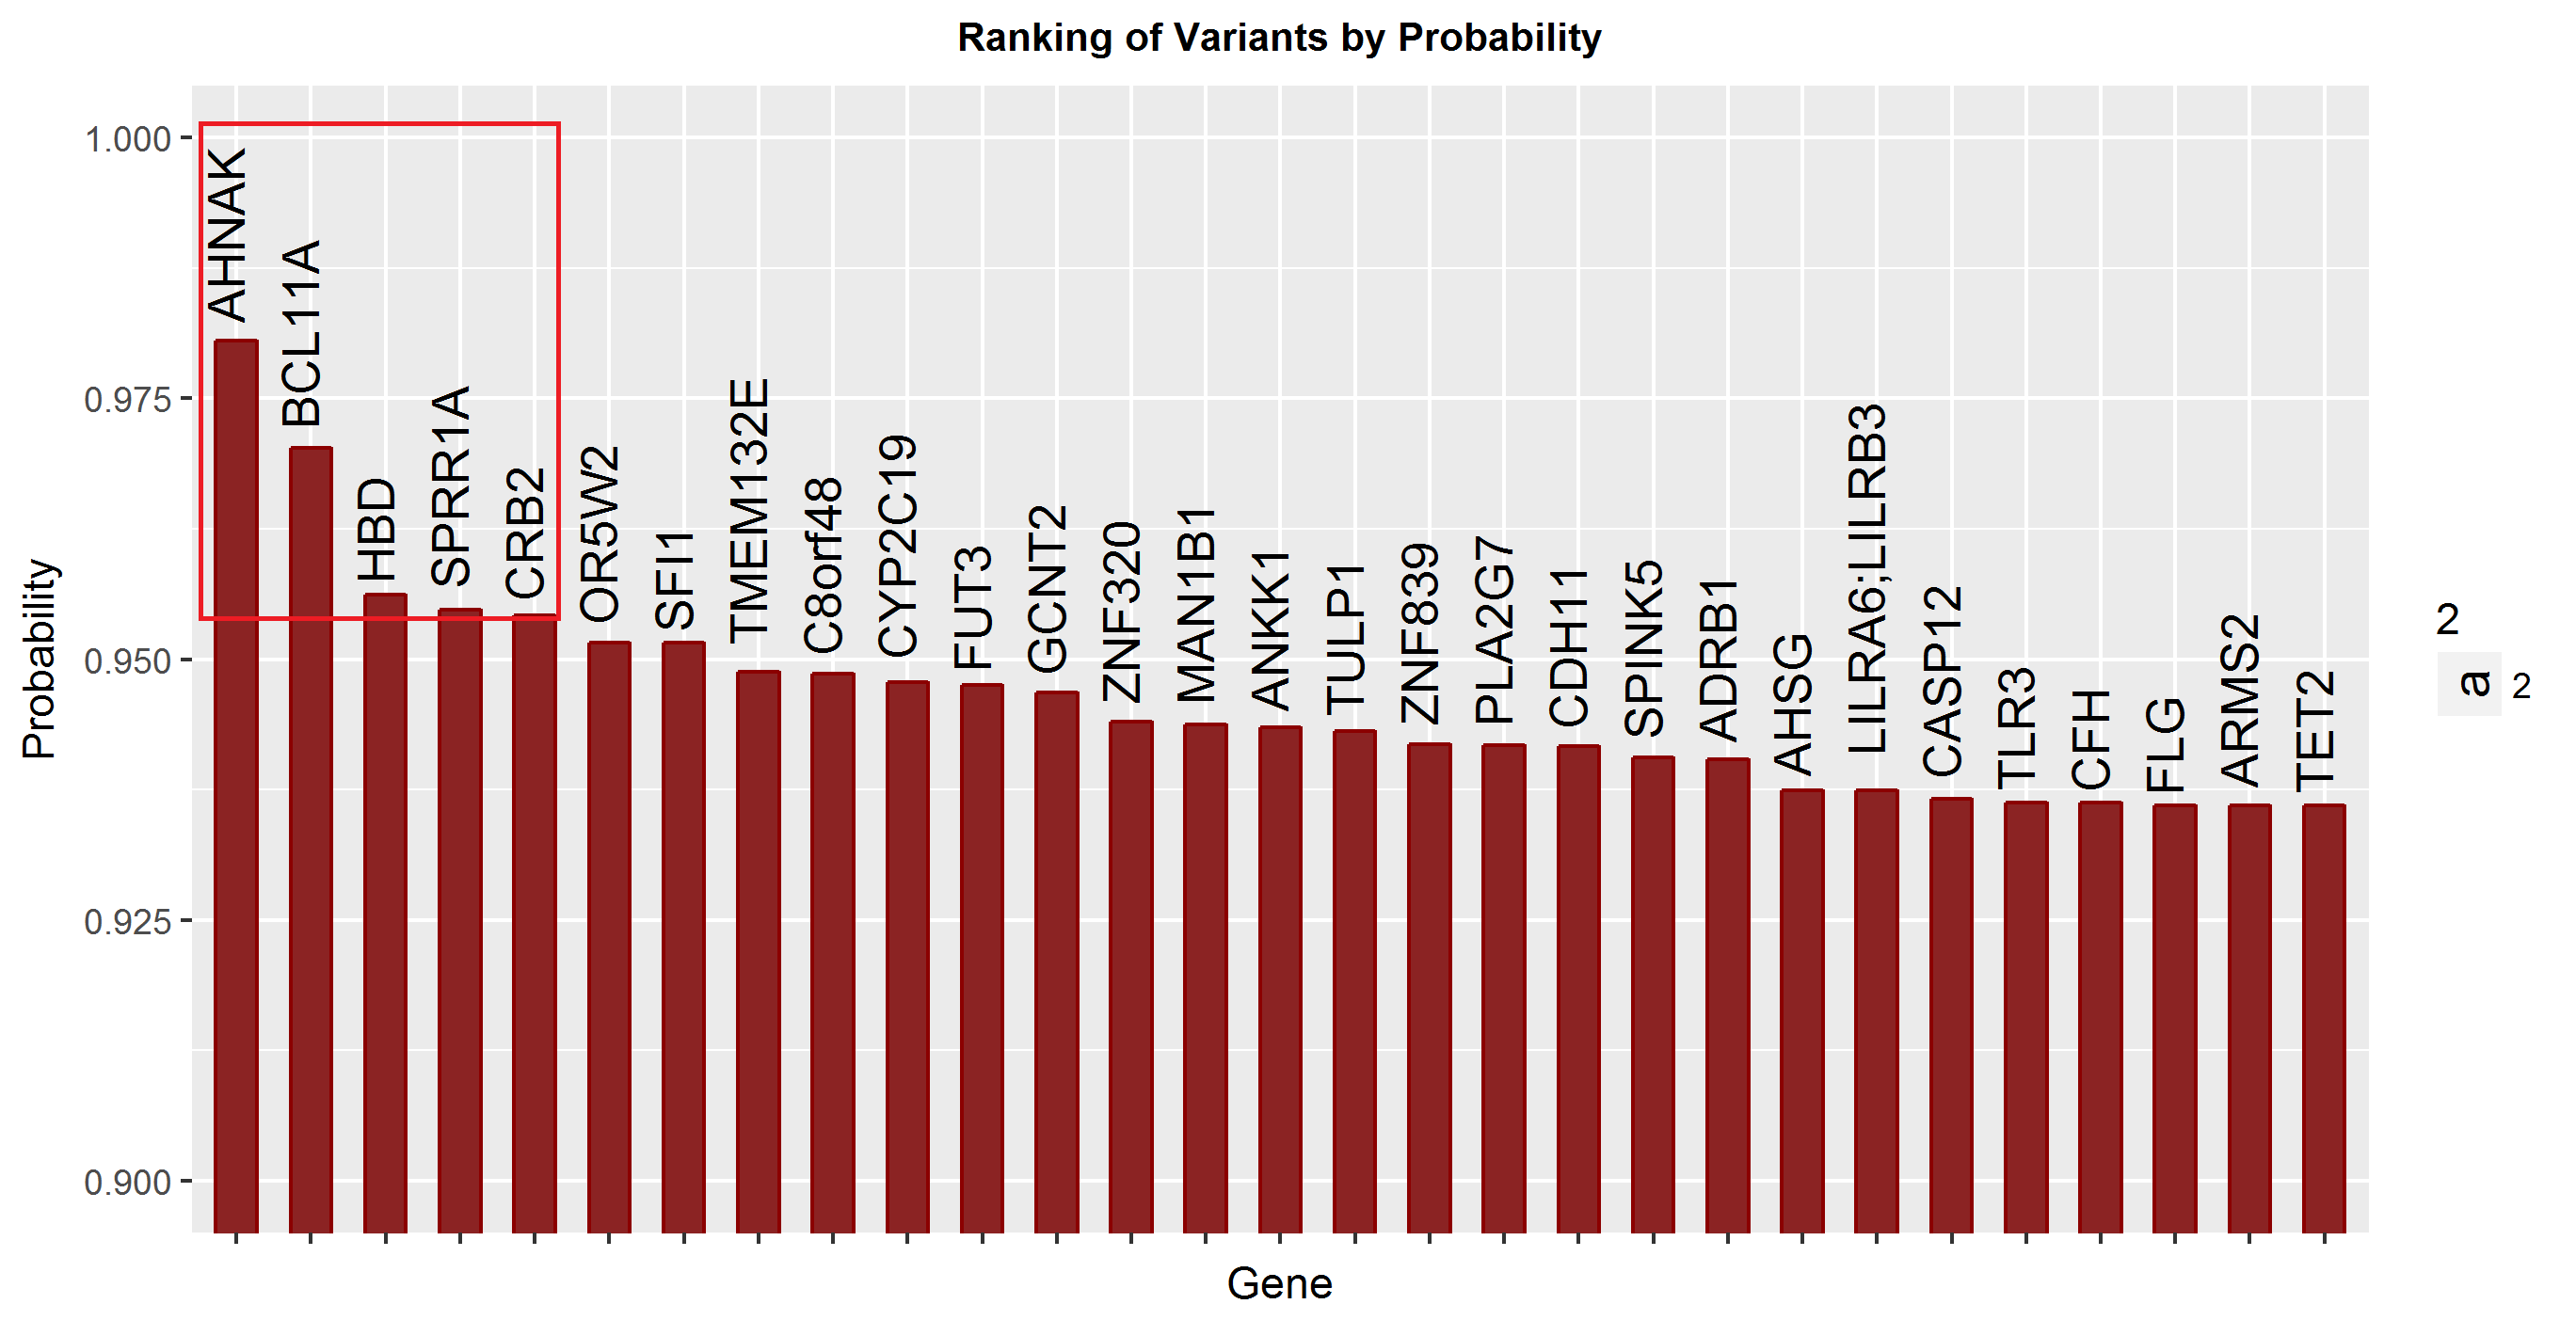
\includegraphics[width=\textwidth]{bayesianranks.png}
\caption{Comparison of Variant Callers}
\centering
\end{figure}

Studying the top 5 genes, we found that four of these five genes have been implicated on lymphomas or other cancers. AHNAK is a known tumour suppressor and has been known to be downregulated inlines of Burkitt Lymphoma. BCL11A is a known proto-oncogene in DLBCL, and has been found to be overexpressed in 75\% of primary mediastinal B-cell Lymphomas, a subset of DLBCL. SPRR1A, the fourth gene ranked in terms of importance, has been shown to be expressed in DLBCL and its expression has been shown to strongly correlate with 5 year survival rate (Figure ). Finally development of B-cell lymphoma has been noted in Crb-2 related syndrome, which is a bi-allelic mutaiton of CRB2. Interestingly, the last highly ranked genes was noted to be a subunit of Hemoglobin. While there is no strong evidence for the role of Hemoglobin in lymphoma, it has been shown to be expressed in aggressive gliobastoma lines, indicating a possible previously unknown role in cancer. This gives us high confidence that the bayesian ranking network is able to pick up important and relevant mutations. Without such a ranking system, we would have to look through over 70 thousand genes, without a way to systematically study their call confidence, as well as their probability of having an effect. 


\begin{figure}[H]
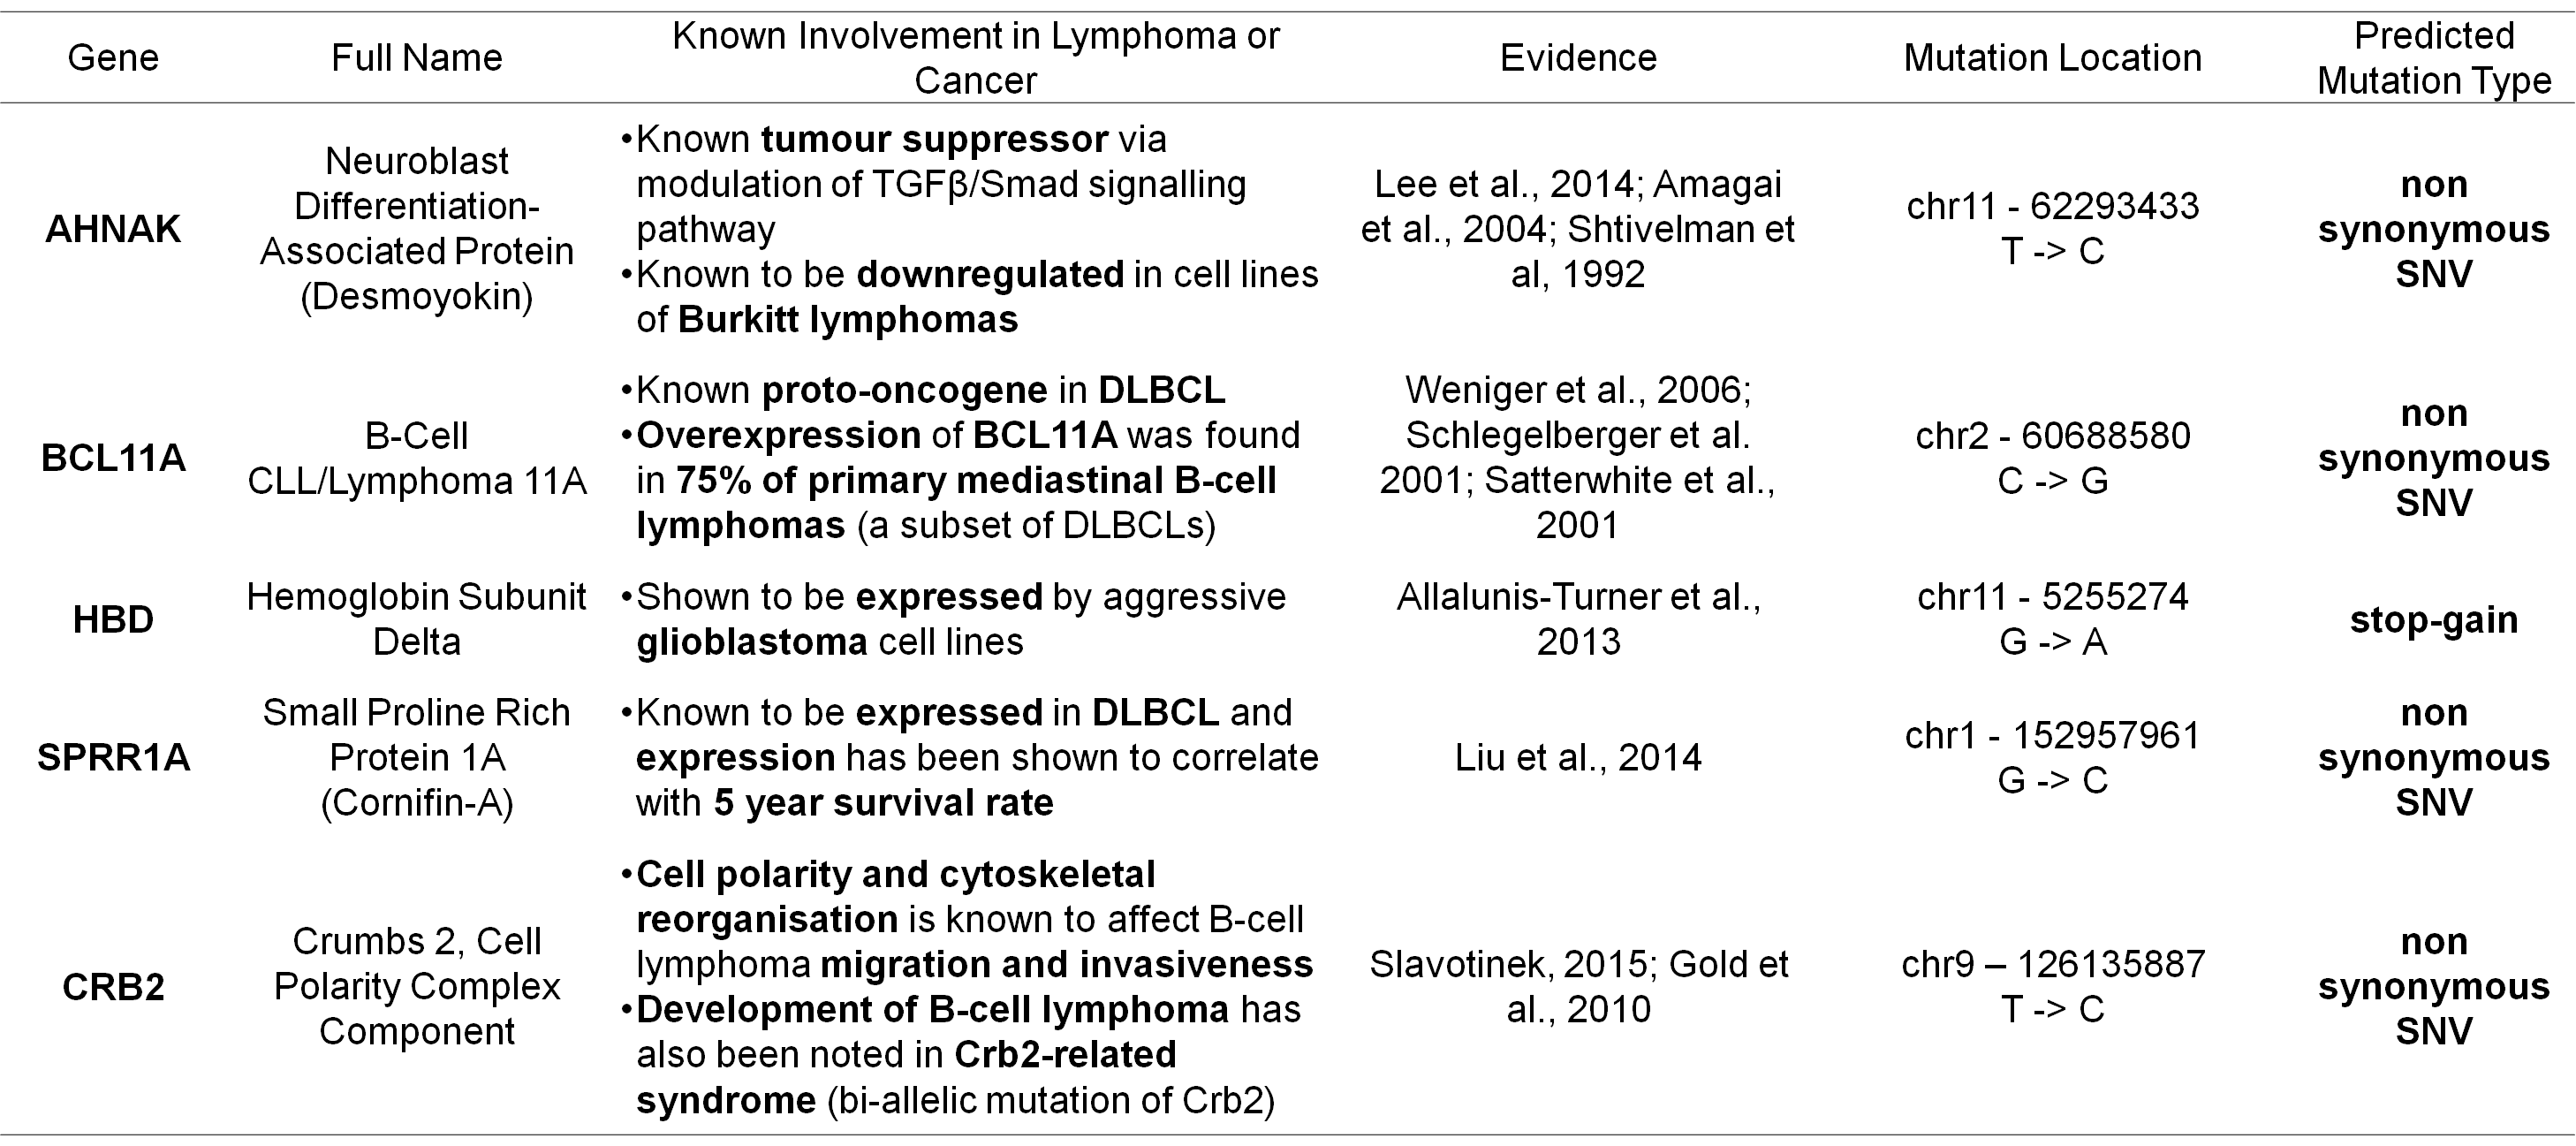
\includegraphics[width=\textwidth]{top5importantgenes.png}
\caption{Comparison of Variant Callers}
\centering
\end{figure}

\begin{figure}[H]
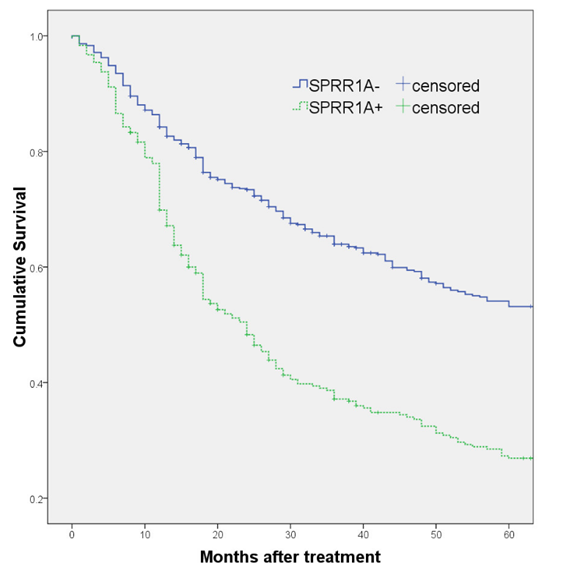
\includegraphics{sprr1adataset.png}
\caption{Comparison of Variant Callers}
\centering
\end{figure}


To aggregate the data from our Bayesian Ranking system, we did a Circos plot for the top 300 genes picked up by our gene ranking system. A Circos enables easy visualisation and analysis of large genome datasets, enabling quick understanding and comprehension of results. From the Ciros Plot (Figure N), we find several interesting gene familes that might also be relevant in B-Cell Lymphoma. These include several Toll-Like Receptors(TLRs), Tlr3 (chr4,rank 26) and Tlr1(chr4,rank 77) as well as interleukin receptors IL4R (chr16,rank 37) and IL1$\beta$ (chr2,rank 196). TLRs are of significant interest in cancer due to their involvement in the caspase pathway, and interleukins are also important in cancer due to their importance in mediating inflammation and immune response. Thus, we show that our bayesian network can be used by Clinicians to quickly interrogate the information from functional annotations and database lookups to understand the disease specifics. 

\begin{figure}[H]
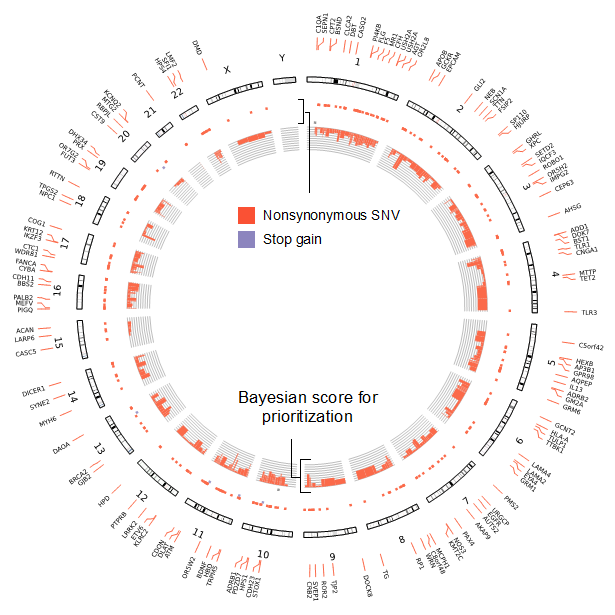
\includegraphics{circosplot.png}
\caption{Comparison of Variant Callers}
\centering
\end{figure}


\section{Summary and Future Directions}


\section{Appendixes}
\subsection{Neural Network Algorithms}

\subsection{Feature Engineering}


\subsection{Mathematical and Statistical Tools}
A. Principal Components Analysis (PCA)\\
Principal Components Analysis (PCA) is a commonly used tool for dimensionality reduce of high dimensional datasets. It was first proposed by Pearson in 1901 (CITATION) and has been commonplace in many data analytics and signal processing methodologies. PCA works by attempting to discover orthogonal principal components (PCs) that are able to represent the original data. Specifically, this means that the PCs are able to capture variance in the datasets. This is done by finding the Eigenvalues and Eigenvectors of the dataset, with the eigenvectors representing a linear combination of all input variables and the eigenvalues representing the amount of variance that that eigenvector is able to represent. Ultimately, we select n eigenvectors that is able to represent a percentage of variance in our dataset. Because each eigenvector is orthogonal, they are able to capture the variance in the dataset. For our analysis, we decided to use 8 principal components - we took the limit as the last principal components that was able to represent at least 0.5\% of variance in the dataset.
 
\begin{figure}[H]
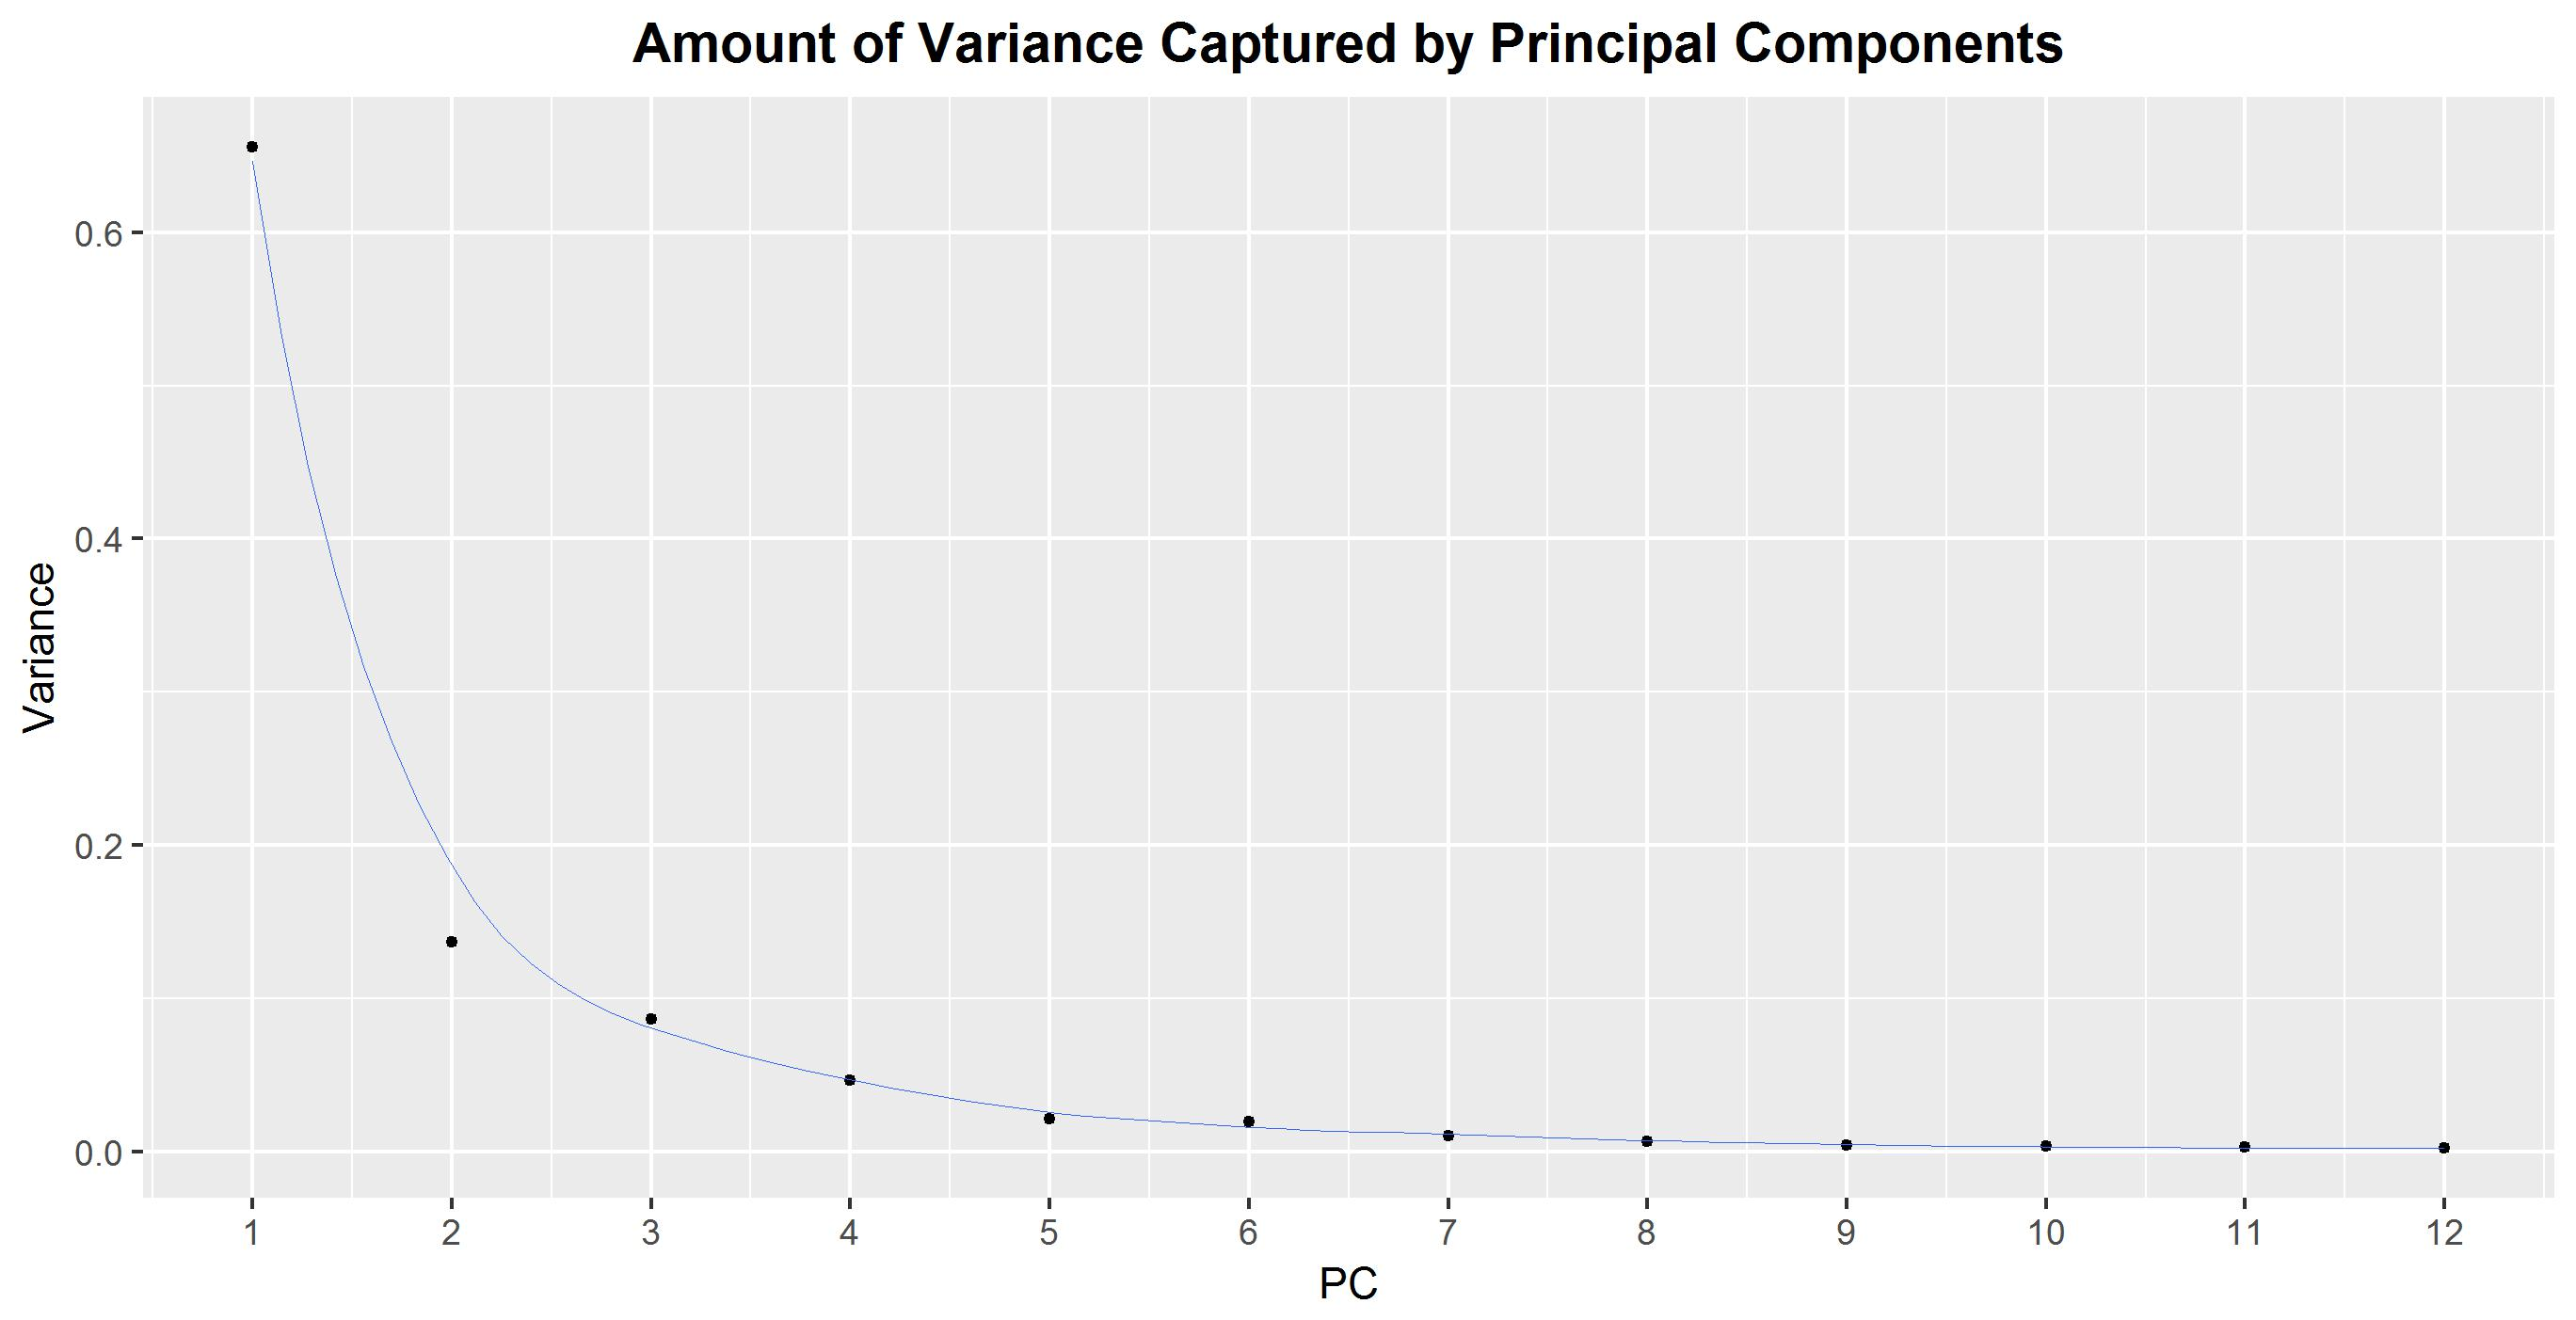
\includegraphics[width=\textwidth]{variancecapturedbypc.jpg}
\caption{Comparison of Variant Callers}
\centering
\end{figure}

To carry out PCA, we used the preprocessing step SciPy to normalise all the input vectors to mean 0 and standard deviation 1. Subsequently, we perform principal components decomposition to obtain the eigenvector transformed representation of the dataset, and their corresponding eigenvalues. We then fit 8 of the principal components that explained the largest amount of variance into the neural network to study if it is able to learn from the compressed representation of the input features. 

B. Synthetic Minority Overrepresentation Technique (SMOTE)
SMOTE is a statistical technique derived in (CITATION) to overcome problems with imbalanced datasets that are common in machine learning. SMOTE oversamples the training class with less variables in a way that tries not to replicate data points (that makes certain data points over-represented) without creating new invalid training training examples. It does this by taking the intersection of two nearest data points of the same training class. This can be seen in Figure N. 

\begin{figure}[H]
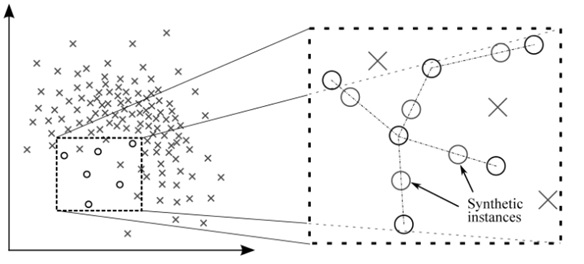
\includegraphics[width=\textwidth]{smoteoversampling.jpg}
\caption{Comparison of Variant Callers}
\centering
\end{figure}

In doing so, it creates a more generalised representation of the sample class with less training examples, without replicating certain datapoints and without creating invalid data. This enables intelligent oversampling of the dataset to balance out the positive and negative feature classes. SMOTE has been shown to be valid for other datasets, including biological data (Figure N). Here, SMOTE was used to accomplish BLANK.

\begin{figure}[H]
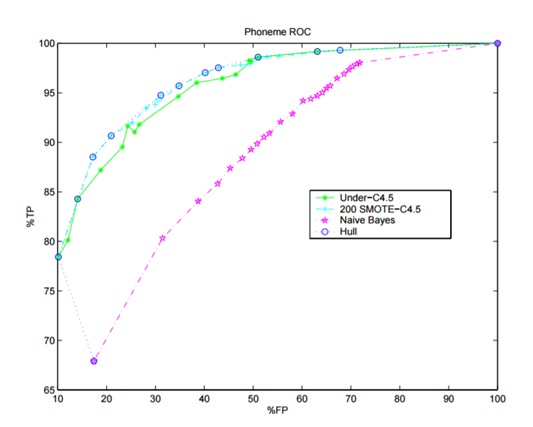
\includegraphics[width=\textwidth]{smoteevidence.jpg}
\caption{Comparison of Variant Callers}
\centering
\end{figure}

\section{Acknowledgements}

\section{Bibilography}

\begin{thebibliography}{9}
\bibitem{latexcompanion} 
O'Rawe, J., Jiang, T., Sun, G., Wu, Y., Wang, W., Hu, J., ... \& Wei, Z. (2013). Low concordance of multiple variant-calling pipelines: practical implications for exome and genome sequencing. Genome medicine, 5(3), 1.
 
\bibitem{einstein} 
 Cornish, A., \& Guda, C. (2015). A comparison of variant calling pipelines using genome in a bottle as a reference. BioMed research international, 2015.

\bibitem{knuthwebsite} 
Mohiyuddin, M., Mu, J. C., Li, J., Asadi, N. B., Gerstein, M. B., Abyzov, A., ... \& Lam, H. Y. (2015). MetaSV: an accurate and integrative structural-variant caller for next generation sequencing. Bioinformatics, btv204.

\bibitem{knuthwebsite} 
Gézsi, A., Bolgár, B., Marx, P., Sarkozy, P., Szalai, C., \& Antal, P. (2015). VariantMetaCaller: automated fusion of variant calling pipelines for quantitative, precision-based filtering. BMC genomics, 16(1), 1.

\bibitem{knuthwebsite} 
Huval, B., Wang, T., Tandon, S., Kiske, J., Song, W., Pazhayampallil, J., Andriluka, M., Rajpurkar, P., Migimatsu, T., Cheng-Yue, R. and Mujica, F., 2015. An empirical evaluation of deep learning on highway driving. arXiv preprint arXiv:1504.01716.

\end{thebibliography}



\end{document}
